\documentclass[12pt, a4paper]{article}

% ── Packages ──────────────────────────────────────────────────────────────────
\usepackage[margin=2.5cm]{geometry}
\usepackage{fontenc}
\usepackage[utf8]{inputenc}
\usepackage{microtype}
\usepackage{setspace}
\usepackage{titlesec}
\usepackage{abstract}
\usepackage{graphicx}
\usepackage{float}
\usepackage{booktabs}
\usepackage{array}
\usepackage{multirow}
\usepackage{amsmath}
\usepackage{amssymb}
\usepackage{natbib}
\usepackage[hidelinks]{hyperref}
\usepackage{xcolor}
\usepackage{caption}
\usepackage{subcaption}
\usepackage{parskip}
\usepackage{lmodern}

% ── Typography ────────────────────────────────────────────────────────────────
\setstretch{1.15}
\setlength{\parskip}{6pt}
\setlength{\parindent}{0pt}

\captionsetup{font=small, labelfont=bf, format=plain, justification=justified}

\titleformat{\section}{\large\bfseries}{\thesection.}{0.5em}{}
\titleformat{\subsection}{\normalsize\bfseries}{\thesubsection}{0.5em}{}
\titlespacing{\section}{0pt}{18pt}{6pt}
\titlespacing{\subsection}{0pt}{10pt}{4pt}

% ── Metadata ──────────────────────────────────────────────────────────────────
\title{\textbf{ERGON: A Quantitative Analysis of Ergativity\\
       Across 180 Languages}}
\author{Roberto Zariquiey\\[4pt]
        \small ERGON Database Project}
\date{2026}

% ══════════════════════════════════════════════════════════════════════════════
\begin{document}
\maketitle
\thispagestyle{empty}

% ── Abstract ──────────────────────────────────────────────────────────────────
\begin{abstract}
\noindent
This report presents a systematic quantitative analysis of ergativity based on
ERGON, a cross-linguistic database of 180 ergative languages across 41 language
families, coded for 24 binary features (GB409\_1--GB409\_24) related to ergative
case marking. Seven analyses are reported: (1)~total ergativity scoring against a
fully-ergative hypothesis template; (2)~conformance to the Silverstein
animacy/person hierarchy; (3)~split ergativity patterns across aspect, tense,
mood, and realis; (4)~pairwise feature correlations using the phi coefficient;
(5)~individual feature predictors of overall ergativity score; (6)~ergativity
dimensionality --- how many conditioning domains a language exploits; and
(7)~phylogenetic signal in feature distributions. Ergative languages score very
high on total ergativity (mean~$= 0.855$, SD~$= 0.144$), the Silverstein
hierarchy is overwhelmingly respected (92.5\% conformance), split ergativity in
unexpected directions is nearly absent ($< 2\%$ per domain), and
tense/aspect/mood/realis features are tightly intercorrelated ($\varphi > 0.97$)
and the strongest individual predictors of ergativity score. Phylogenetic signal
is moderate-to-large ($\eta^2 \approx 0.41$), confirming that ergativity is
partly but not entirely genealogically determined.

\medskip\noindent
\textbf{Keywords:} ergativity, typology, Silverstein hierarchy, split ergativity,
phylogenetic signal, CLDF, quantitative linguistics
\end{abstract}

\newpage
\tableofcontents
\newpage

% ══════════════════════════════════════════════════════════════════════════════
\section{Introduction}

Ergativity --- the grammatical pattern in which the agent of an intransitive verb
(\textsc{s}) is treated like the patient of a transitive verb (\textsc{p}) rather
than like the agent (\textsc{a}) --- is one of the most theoretically debated
phenomena in linguistic typology. Despite a rich tradition of qualitative
description \citep{dixon1994, comrie1978, manning1996}, large-scale quantitative
studies of ergativity remain scarce, largely due to the absence of standardised
cross-linguistic databases covering the full range of ergative phenomena.

ERGON addresses this gap. It codes 24 binary features for 180 ergative languages,
organised in Cross-Linguistic Data Format \citep[CLDF;][]{forkel2018} for full
reproducibility. The features cover: the presence of an overt absolutive marker;
ergative alignment on first, second, and third person pronouns and on full NPs;
ergative alignment conditioned by aspect, tense, mood, realis status, agentivity,
topicality, animacy, and clause type; and the formal overlap of the ergative
marker with the genitive or instrumental.

This report presents results from seven quantitative analyses conducted on the
current ERGON release. Our goals are both descriptive --- to establish the
typological landscape of ergativity as encoded in ERGON --- and theoretical,
testing specific hypotheses about hierarchy effects, split patterns, feature
co-occurrence, and phylogenetic signal.

% ══════════════════════════════════════════════════════════════════════════════
\section{Data}

ERGON currently covers 180 ergative languages drawn from 41 language families
across all inhabited continents. The database includes 4,057 coded binary values
(0~= feature absent, 1~= feature present) across the 24 GB409 features, after
excluding missing-value entries coded as `?'. All data are stored in CLDF
StructureDataset format, with separate tables for languages, parameters, and
values, allowing straightforward integration with other CLDF-compatible resources
such as Glottolog and WALS.

% ══════════════════════════════════════════════════════════════════════════════
\section{Analysis 1: Total Ergativity Score}

\subsection{Method}

Following \citet{greenhill2010} and \citet{blasi2019}, we define a
`fully ergative' hypothesis template specifying the expected value (0 or 1) for
each feature under full ergativity. The template was derived from an
expert-annotated coding guide. For each language, we compute an ergativity score
as the proportion of template-relevant features for which the language matches the
prediction, restricted to languages with data on at least 12 of the relevant
features. This yields a continuous score in $[0, 1]$.

\subsection{Results}

169 languages had sufficient data for scoring. Ergativity scores are high overall
($M = 0.855$, $SD = 0.144$, $\mathrm{Mdn} = 0.900$), confirming that ERGON
languages are prototypically ergative across the full range of coded features.
Sixteen languages achieved a perfect score of 1.0 --- ergative marking present
across all coded features --- including Guiqiong, Dzongkha, Chukchi, Coeur
d'Alene, and Kalkatungu.

At the family level, Pama-Nyungan shows the highest mean ergativity
($M = 0.891$, $n = 21$), followed by Trans-Himalayan ($M = 0.853$, $n = 42$) and
Eskimo-Aleut ($M = 0.844$, $n = 3$). Austronesian languages show the greatest
internal heterogeneity and the lowest mean among well-represented families
($M = 0.677$, $n = 31$), reflecting the typological diversity within this large
genealogical unit. Indo-European ($M = 0.805$) and Nakh-Daghestanian
($M = 0.803$) also pattern below the overall mean.

\begin{figure}[H]
  \centering
  
\includegraphics[width=0.78\textwidth]{figures/fig1_score_distribution.png}
  \caption{Distribution of ergativity scores across 169 ergative languages with
    sufficient data. Dashed line~= mean (0.855); dotted line~= median (0.900).}
  \label{fig:score_dist}
\end{figure}

\begin{figure}[H]
  \centering
  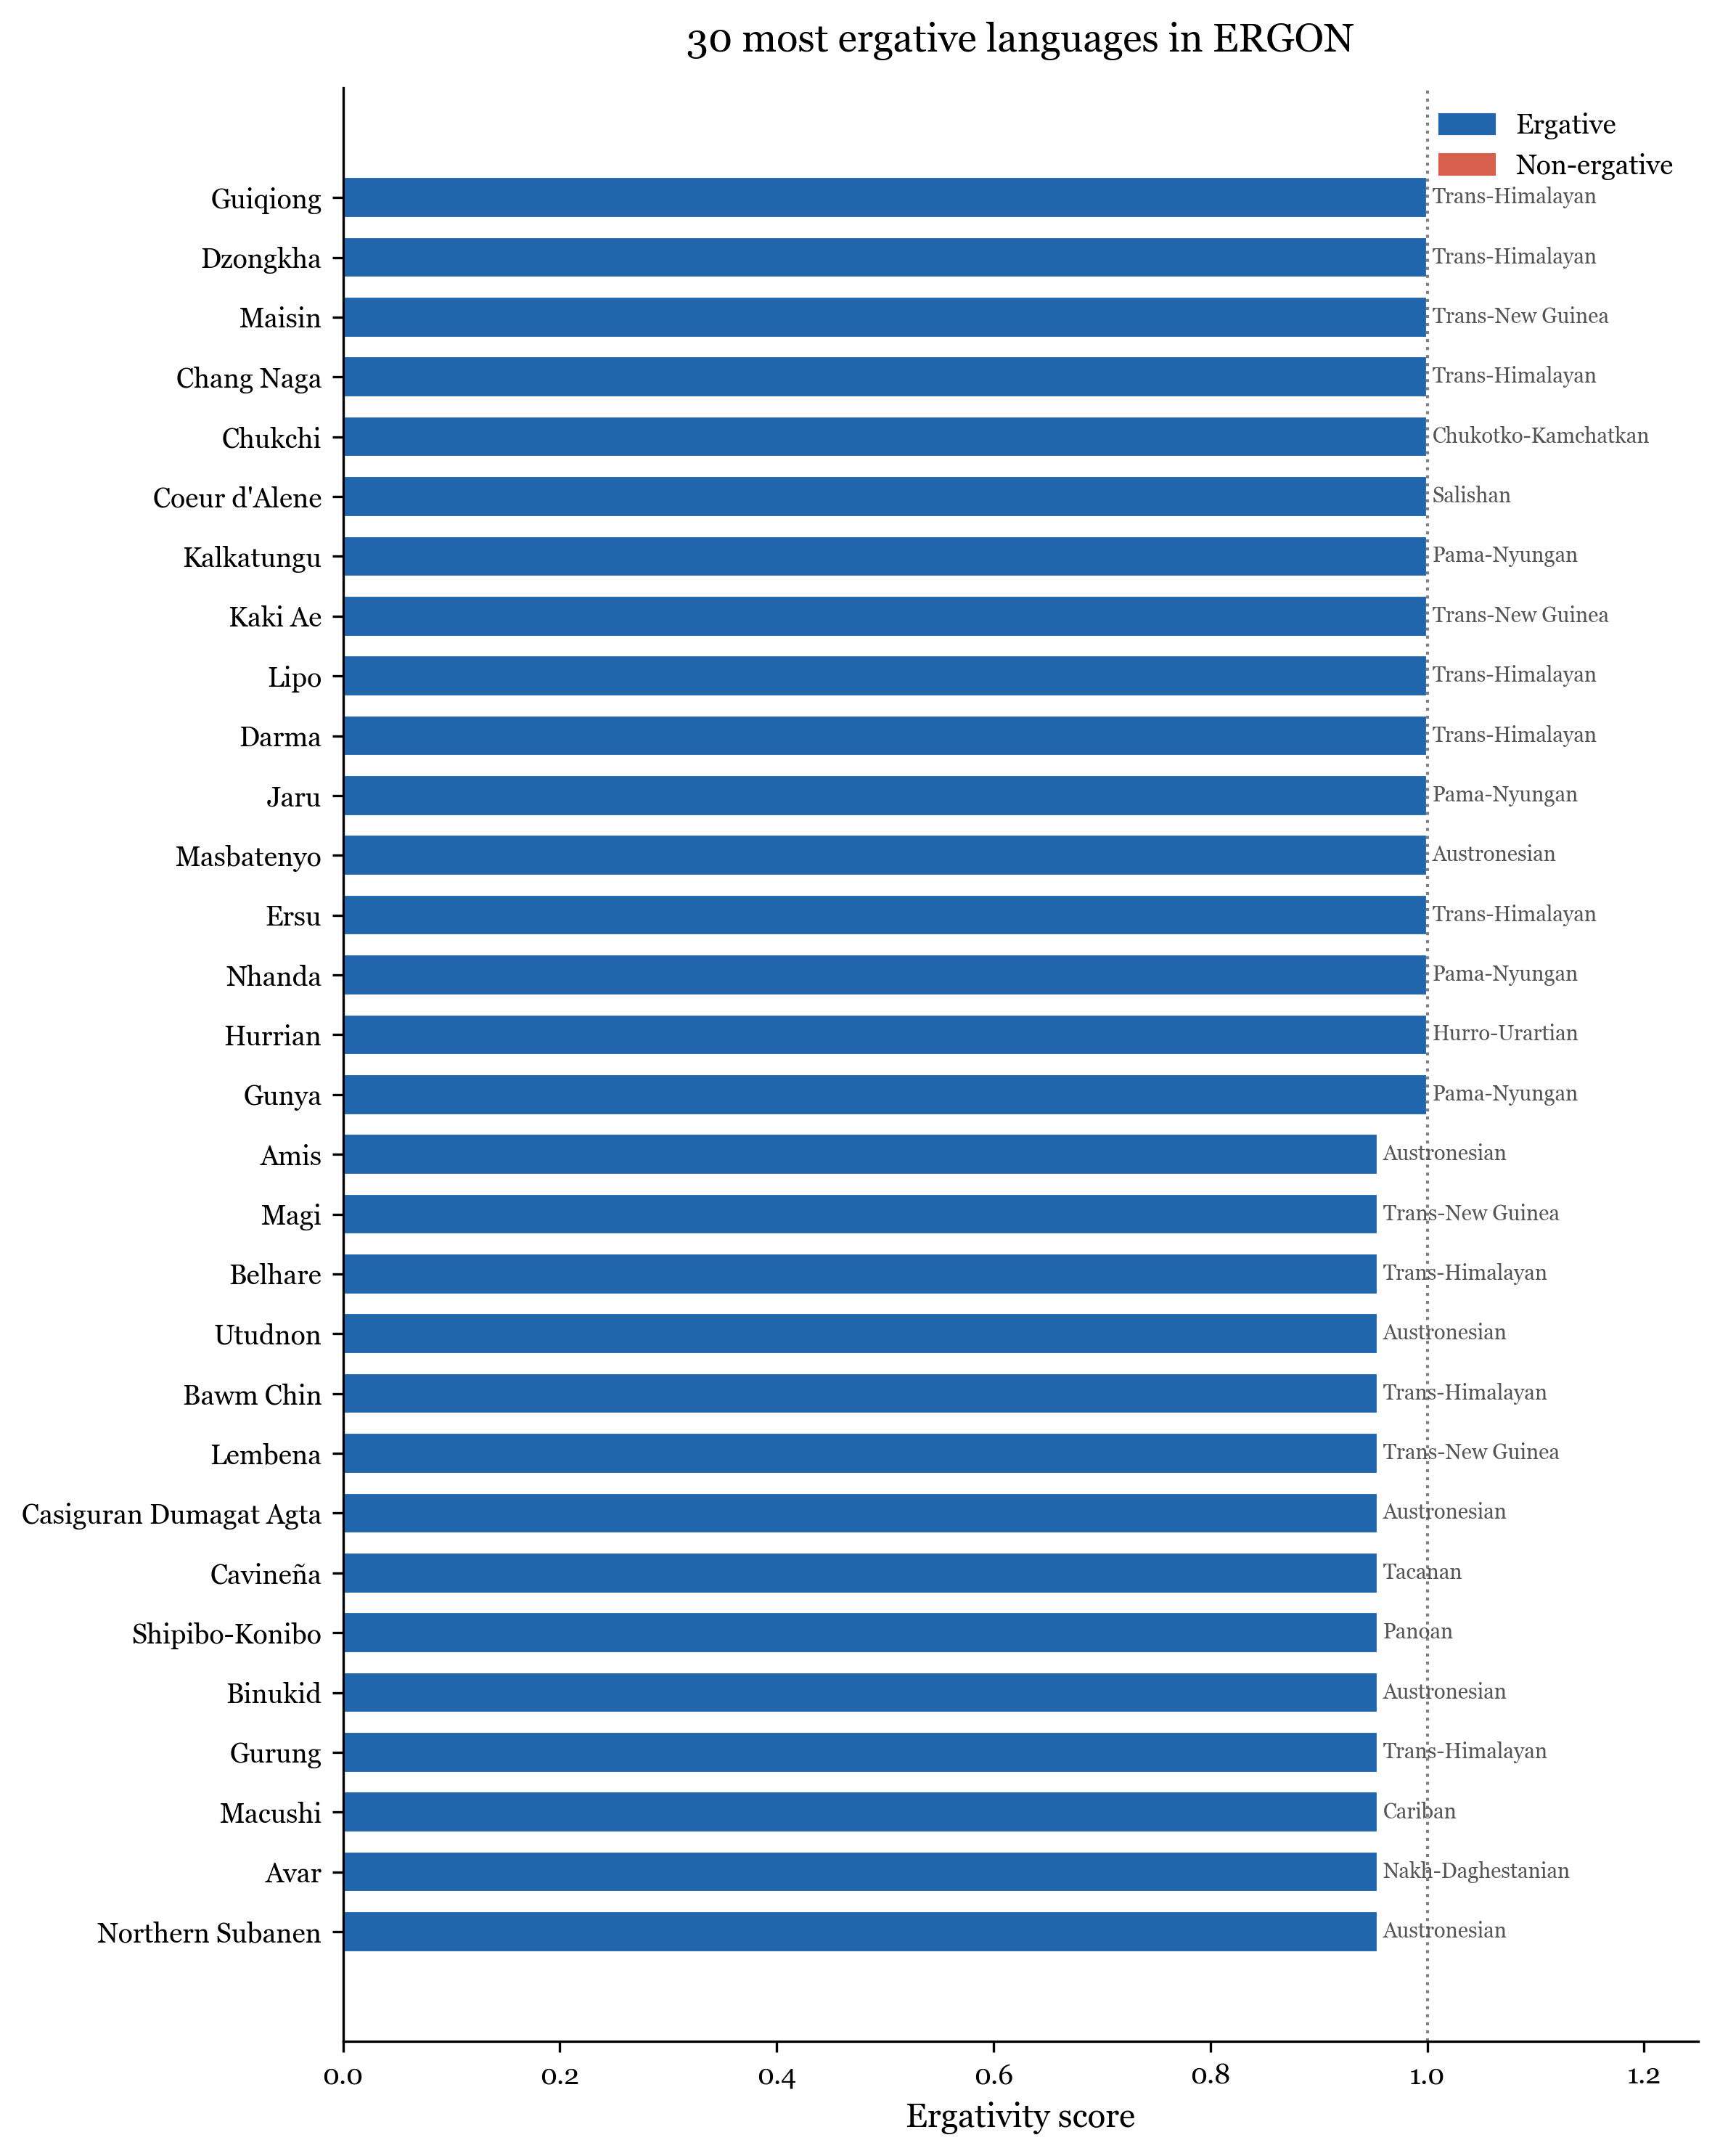
\includegraphics[width=0.68\textwidth]{figures/fig2_top30.png}
  \caption{The 30 highest-scoring languages in ERGON, annotated by family.}
  \label{fig:top30}
\end{figure}

\begin{figure}[H]
  \centering
  
\includegraphics[width=0.85\textwidth]{figures/fig3_families.png}
  \caption{Ergativity score distributions by language family (families with
    $\geq 3$ languages). Red dashed line~= overall mean (0.855).}
  \label{fig:families}
\end{figure}

\begin{figure}[H]
  \centering
  
\includegraphics[width=0.85\textwidth]{figures/fig4_feature_profile.png}
  \caption{Proportion of ergative languages with each feature coded as 1
    (present).}
  \label{fig:feature_profile}
\end{figure}

% ══════════════════════════════════════════════════════════════════════════════
\section{Analysis 2: Silverstein Animacy/Person Hierarchy}

\subsection{Method}

The Silverstein hierarchy \citep{silverstein1976, dixon1979} predicts that
ergative case marking should form an implicational scale across person/animacy:
if a language marks the ergative on a category higher on the hierarchy (towards
1st person), it should also mark it on all lower categories (towards full NPs).
ERGON features GB409\_2--GB409\_5 encode ergative marking on first person, second
person, third person, and full NPs respectively. We classify each language into
one of five valid patterns or as a hierarchy violation.

Valid patterns are: \textsc{none}~$[0,0,0,0]$; \textsc{hier3} (NPs only,
$[0,0,0,1]$); \textsc{hier2} (3rd person + NPs, $[0,0,1,1]$); \textsc{hier1}
(2nd--3rd person + NPs, $[0,1,1,1]$); and \textsc{hier4} (all persons + NPs,
$[1,1,1,1]$). Any other combination counts as a violation.

\subsection{Results}

Of 160 ergative languages with complete data on all four features, 148 (92.5\%)
conform to the Silverstein hierarchy. The most common pattern is \textsc{hier4}
--- ergative marking across all persons and NPs --- attested in 103 languages
(64.4\%). \textsc{Hier3} (NPs only) is the next most common (23 languages,
14.4\%), followed by \textsc{hier2} (3rd person + NPs, $n = 16$, 10.0\%) and
\textsc{hier1} (2nd--3rd person + NPs, $n = 4$, 2.5\%). Two languages show no
ergative person marking.

Twelve languages (7.5\%) violate the hierarchy. The most common violation pattern
is $[1,1,1,0]$ --- ergative on all persons but not on full NPs --- found in three
Austronesian languages (Pitu Ulunna Salu, Bugis, Mag-anchi Agta) and one
Pama-Nyungan language (Narungga). Kabardian (Northwest Caucasian), Hunzib
(Nakh-Daghestanian), and Japhug (Trans-Himalayan) show pattern $[0,0,1,0]$ ---
3rd person only, skipping NPs. Karitiana (Tupian) is the most extreme violator:
$[1,0,0,0]$ --- ergative only on 1st person.

\begin{figure}[H]
  \centering
  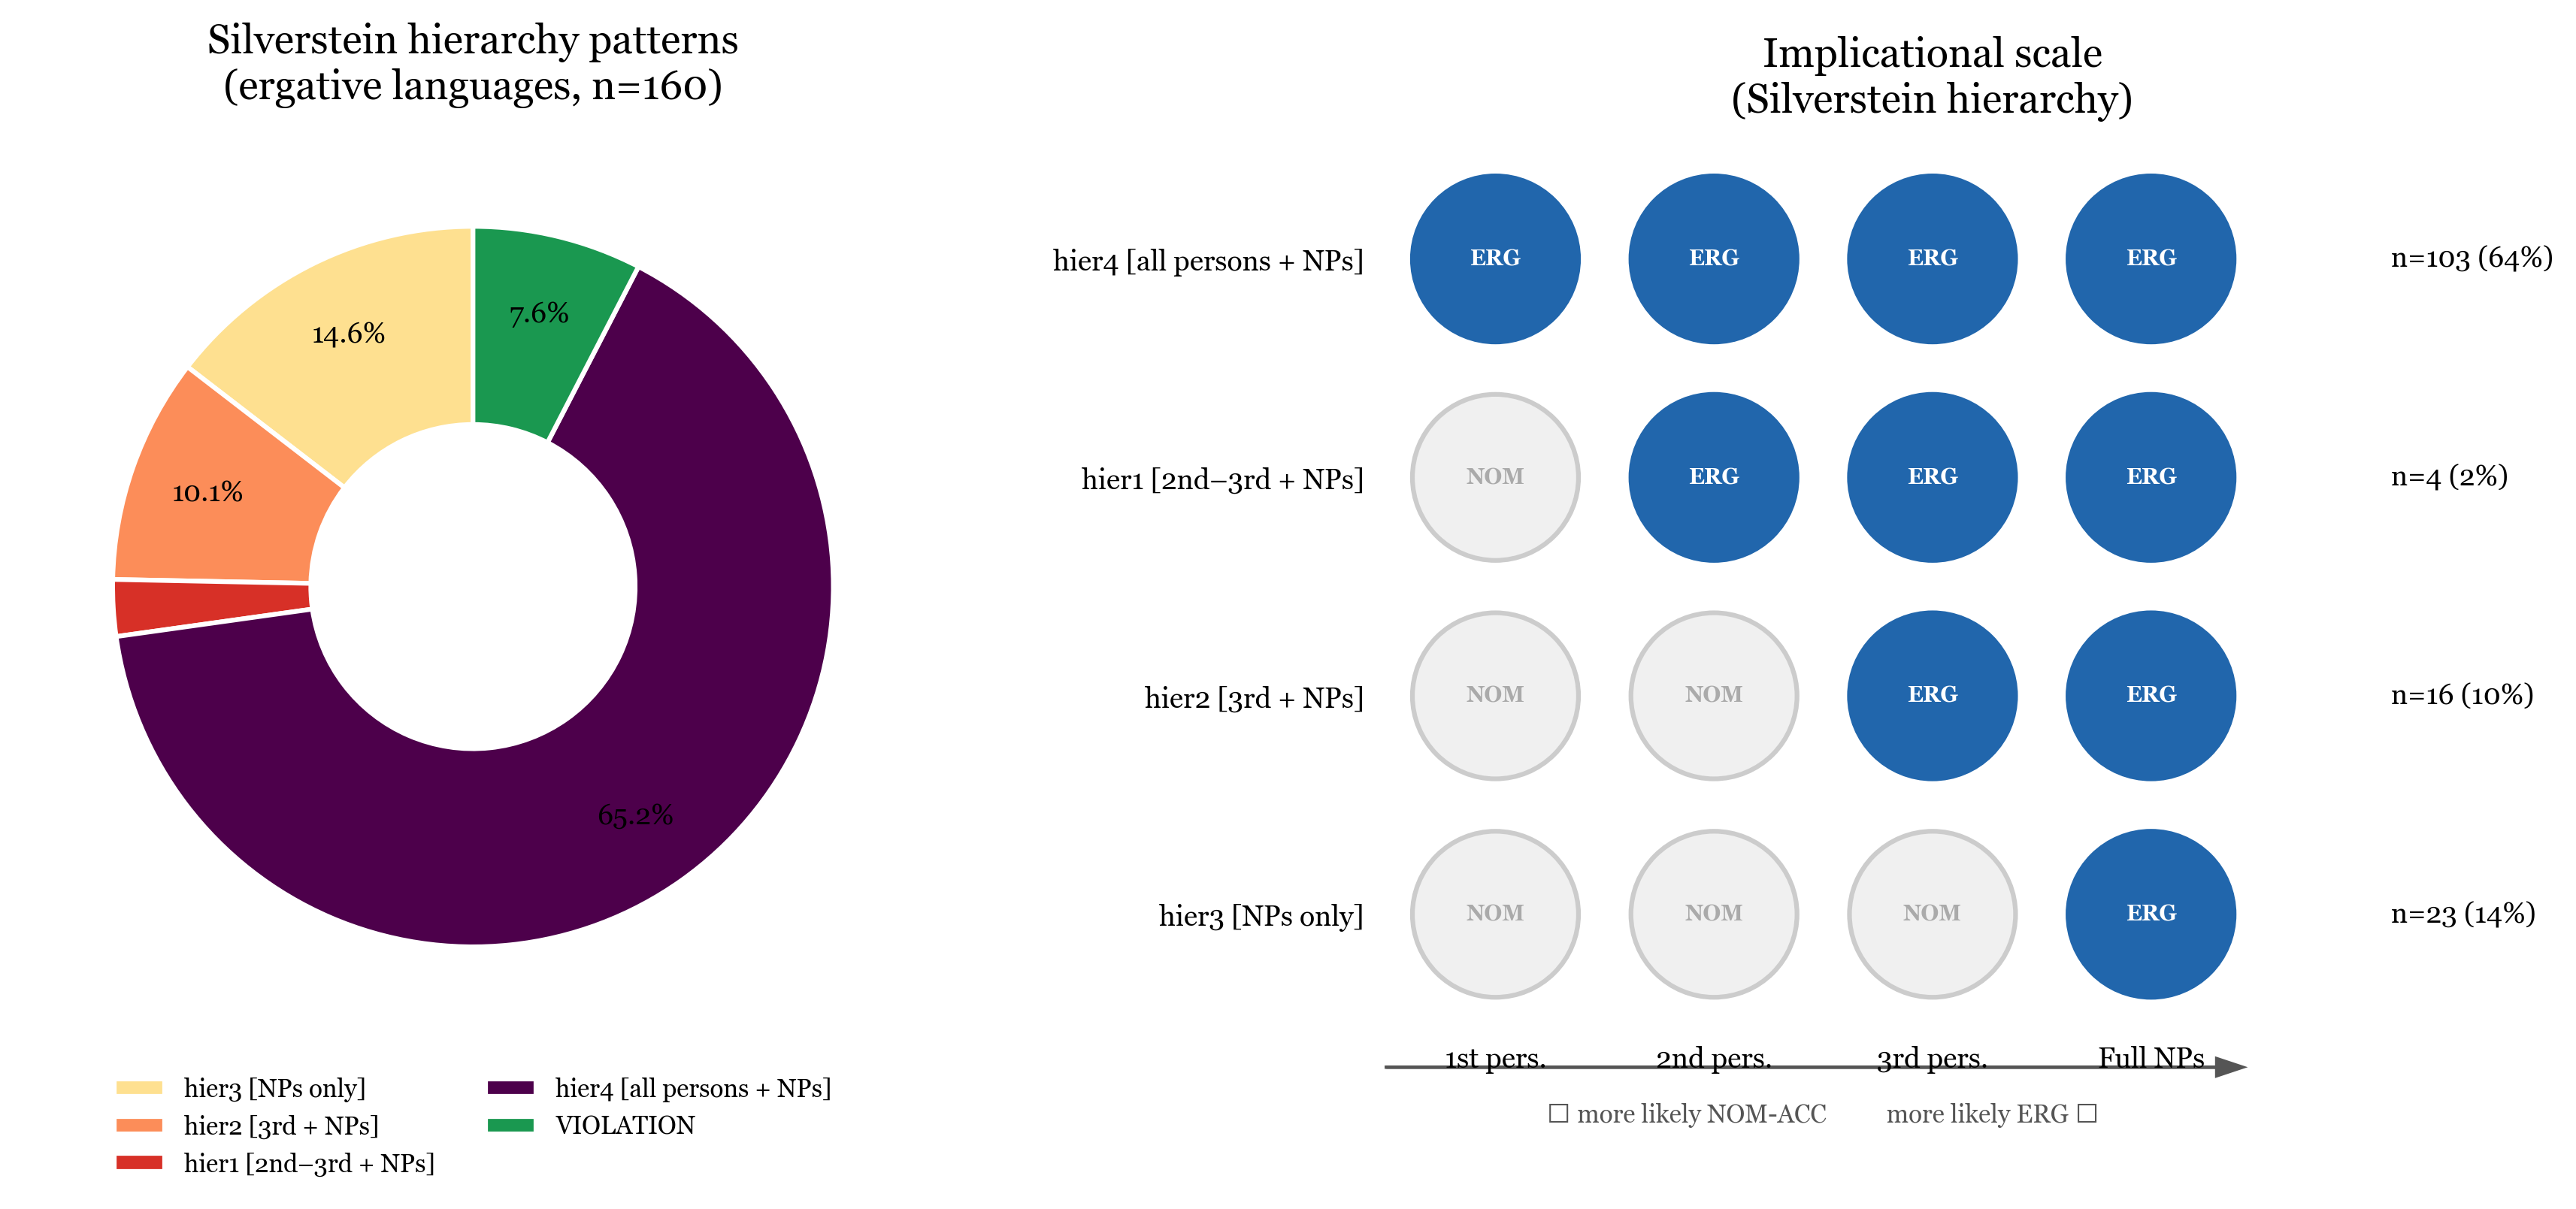
\includegraphics[width=0.88\textwidth]{figures/fig5_silverstein_patterns.png}
  \caption{Left: distribution of Silverstein hierarchy patterns among ergative
    languages. Right: implicational scale diagram with $n$ and \% for each valid
    pattern.}
  \label{fig:silverstein}
\end{figure}

\begin{figure}[H]
  \centering
  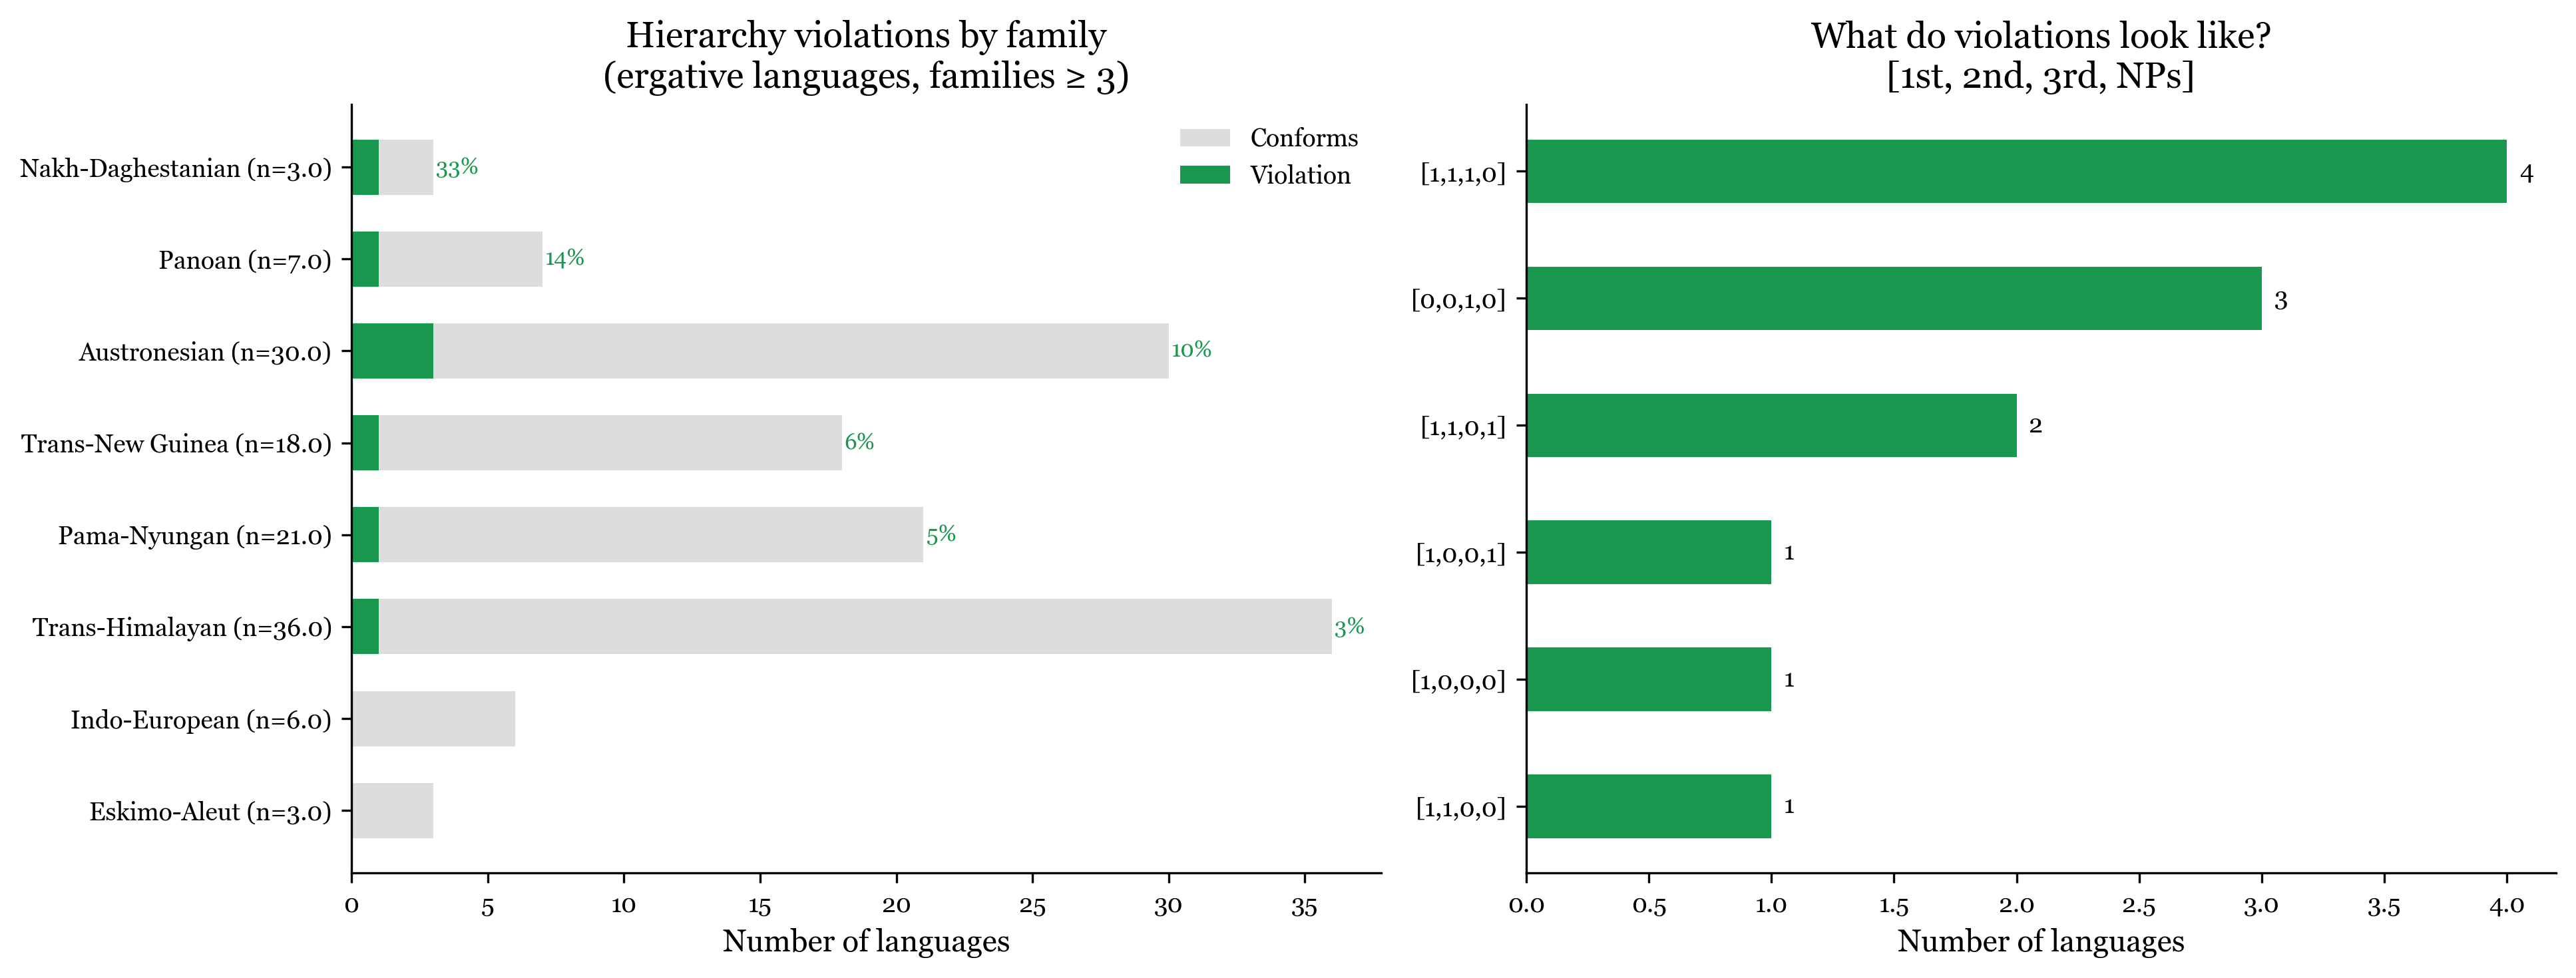
\includegraphics[width=0.88\textwidth]{figures/fig6_violations.png}
  \caption{Left: violation rates by family (families $\geq 3$ languages). Right:
    violation pattern types $[1\text{st},\ 2\text{nd},\ 3\text{rd},\ \text{NPs}]$.}
  \label{fig:violations}
\end{figure}

\begin{figure}[H]
  \centering
  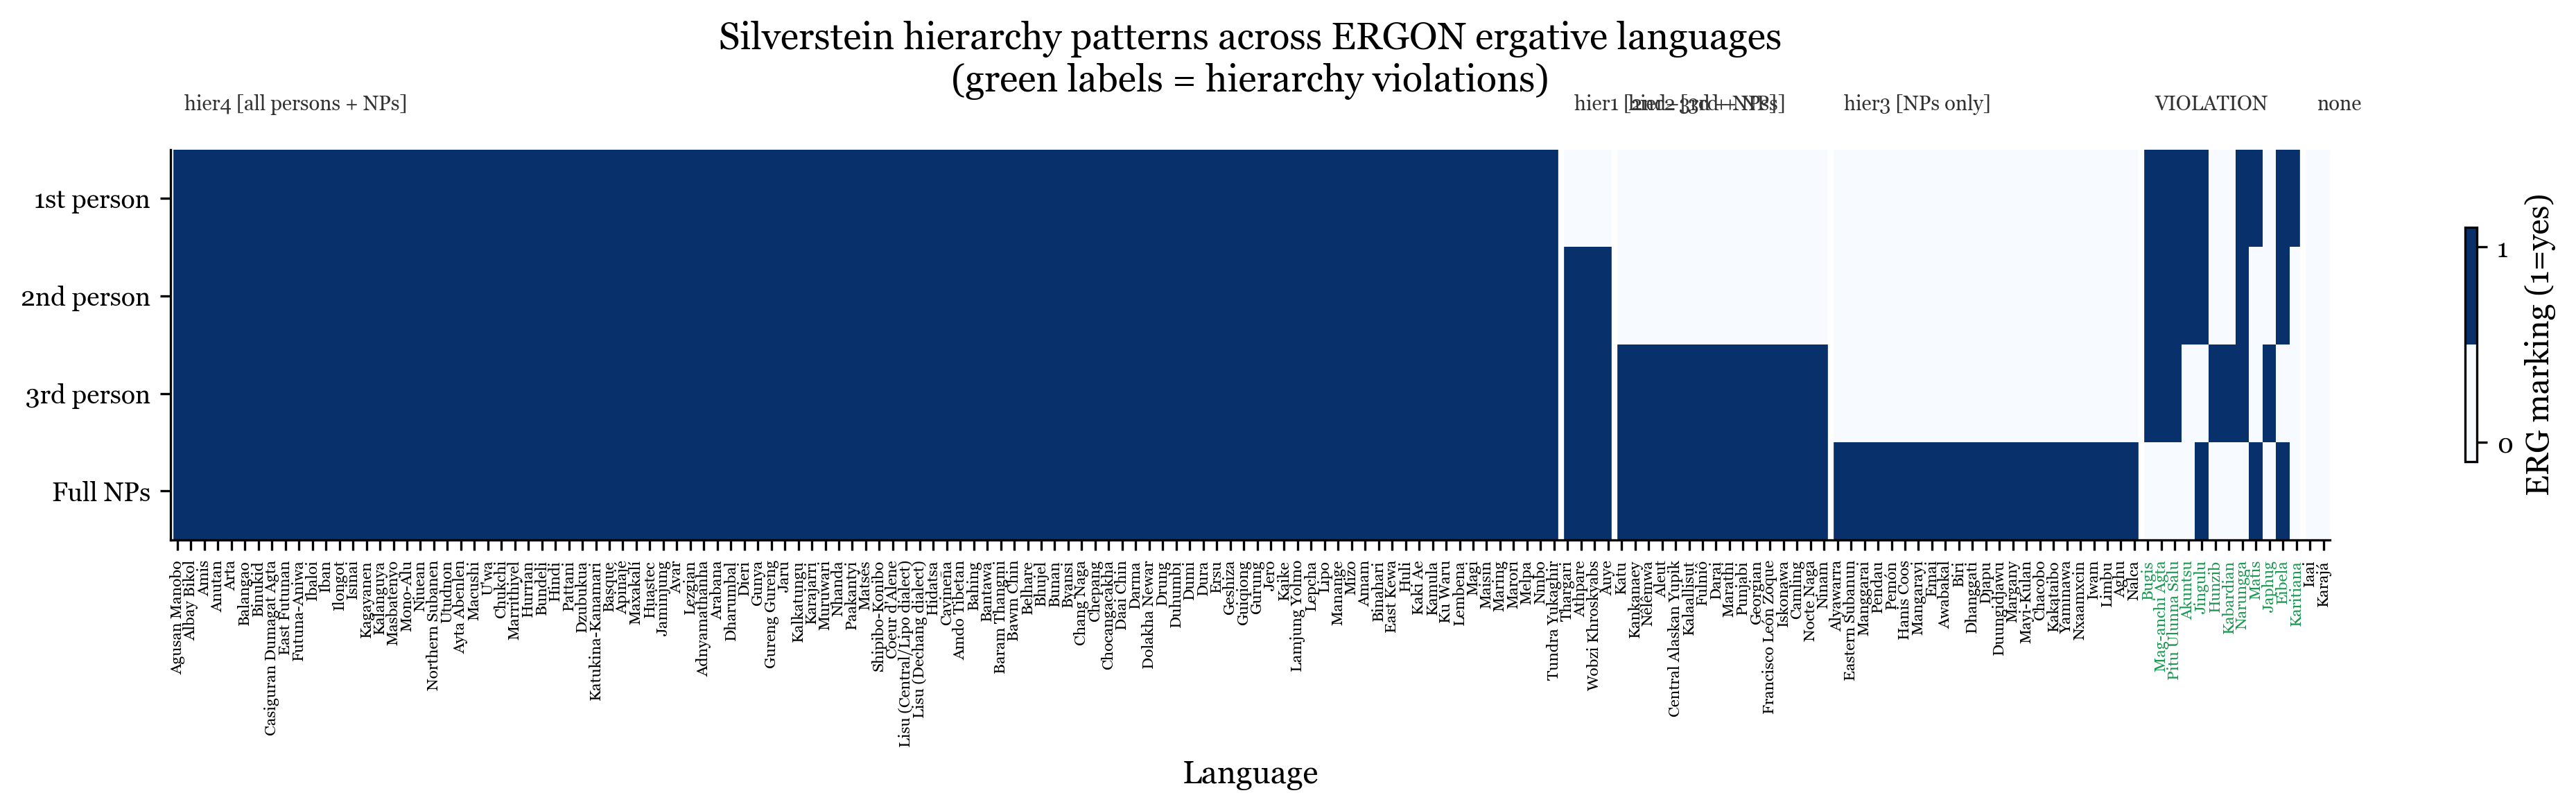
\includegraphics[width=0.95\textwidth]{figures/fig7_heatmap.png}
  \caption{Heatmap of ergative marking across all ergative languages for the four
    Silverstein features. Languages with violations are labelled in green.}
  \label{fig:heatmap}
\end{figure}

% ══════════════════════════════════════════════════════════════════════════════
\section{Analysis 3: Split Ergativity Patterns}

\subsection{Method}

Split ergativity refers to languages in which ergative alignment is restricted to
specific grammatical contexts. \citet{dixon1994} and \citet{givon2001} identify
aspect (\textsc{perf} $>$ \textsc{impf}), tense (\textsc{past} $>$
\textsc{non-past}), mood (\textsc{ind} $>$ \textsc{non-ind}), and realis
(\textsc{real} $>$ \textsc{irr}) as the classic conditioning environments, each
predicting a specific typological direction. ERGON codes each context as a
separate binary feature, allowing us to test both the expected and unexpected
directions. For each of the four domains, we classify ergative languages into:
uniform \textsc{erg} (both~= 1), uniform \textsc{nom-acc} (both~= 0), expected
split, unexpected split, or other.

\subsection{Results}

The overwhelming finding is uniformity: across all four domains, approximately
91\% of languages with relevant data show ergative marking in both contexts
(uniform \textsc{erg}):

\begin{table}[H]
\centering
\caption{Split ergativity pattern counts by conditioning domain.}
\label{tab:splits}
\begin{tabular}{lrrrrrr}
\toprule
Domain & $n$ & Uniform ERG & Expected split & Unexpected split & Uniform NOM-ACC \\
\midrule
Aspect  & 139 & 126 (90.6\%) & 7 (5.0\%) & 2 (1.4\%) & 4 (2.9\%) \\
Tense   & 152 & 139 (91.4\%) & 7 (4.6\%) & 1 (0.7\%) & 5 (3.3\%) \\
Mood    & 134 & 123 (91.8\%) & 7 (5.2\%) & 0 (0.0\%) & 4 (3.0\%) \\
Realis  & 132 & 120 (90.9\%) & 7 (5.3\%) & 0 (0.0\%) & 5 (3.8\%) \\
\bottomrule
\end{tabular}
\end{table}

Expected splits (the classic Dixonian pattern) exist but are rare. Unexpected
splits are nearly absent: only two languages show an unexpected split in any
domain --- Emai (Niger-Congo) and Karitiana (Tupian). These results suggest that
in ERGON languages, ergativity is predominantly a pervasive structural property
rather than a context-restricted one.

\begin{figure}[H]
  \centering
  
\includegraphics[width=0.88\textwidth]{figures/fig8_splits_overview.png}
  \caption{Split ergativity patterns across the four conditioning domains. Each
    bar represents 100\% of languages with data in that domain.}
  \label{fig:splits_overview}
\end{figure}

\begin{figure}[H]
  \centering
  
\includegraphics[width=0.82\textwidth]{figures/fig9_splits_families.png}
  \caption{Families with unexpected splits, shown as \% of ergative languages
    per family.}
  \label{fig:splits_families}
\end{figure}

\begin{figure}[H]
  \centering
  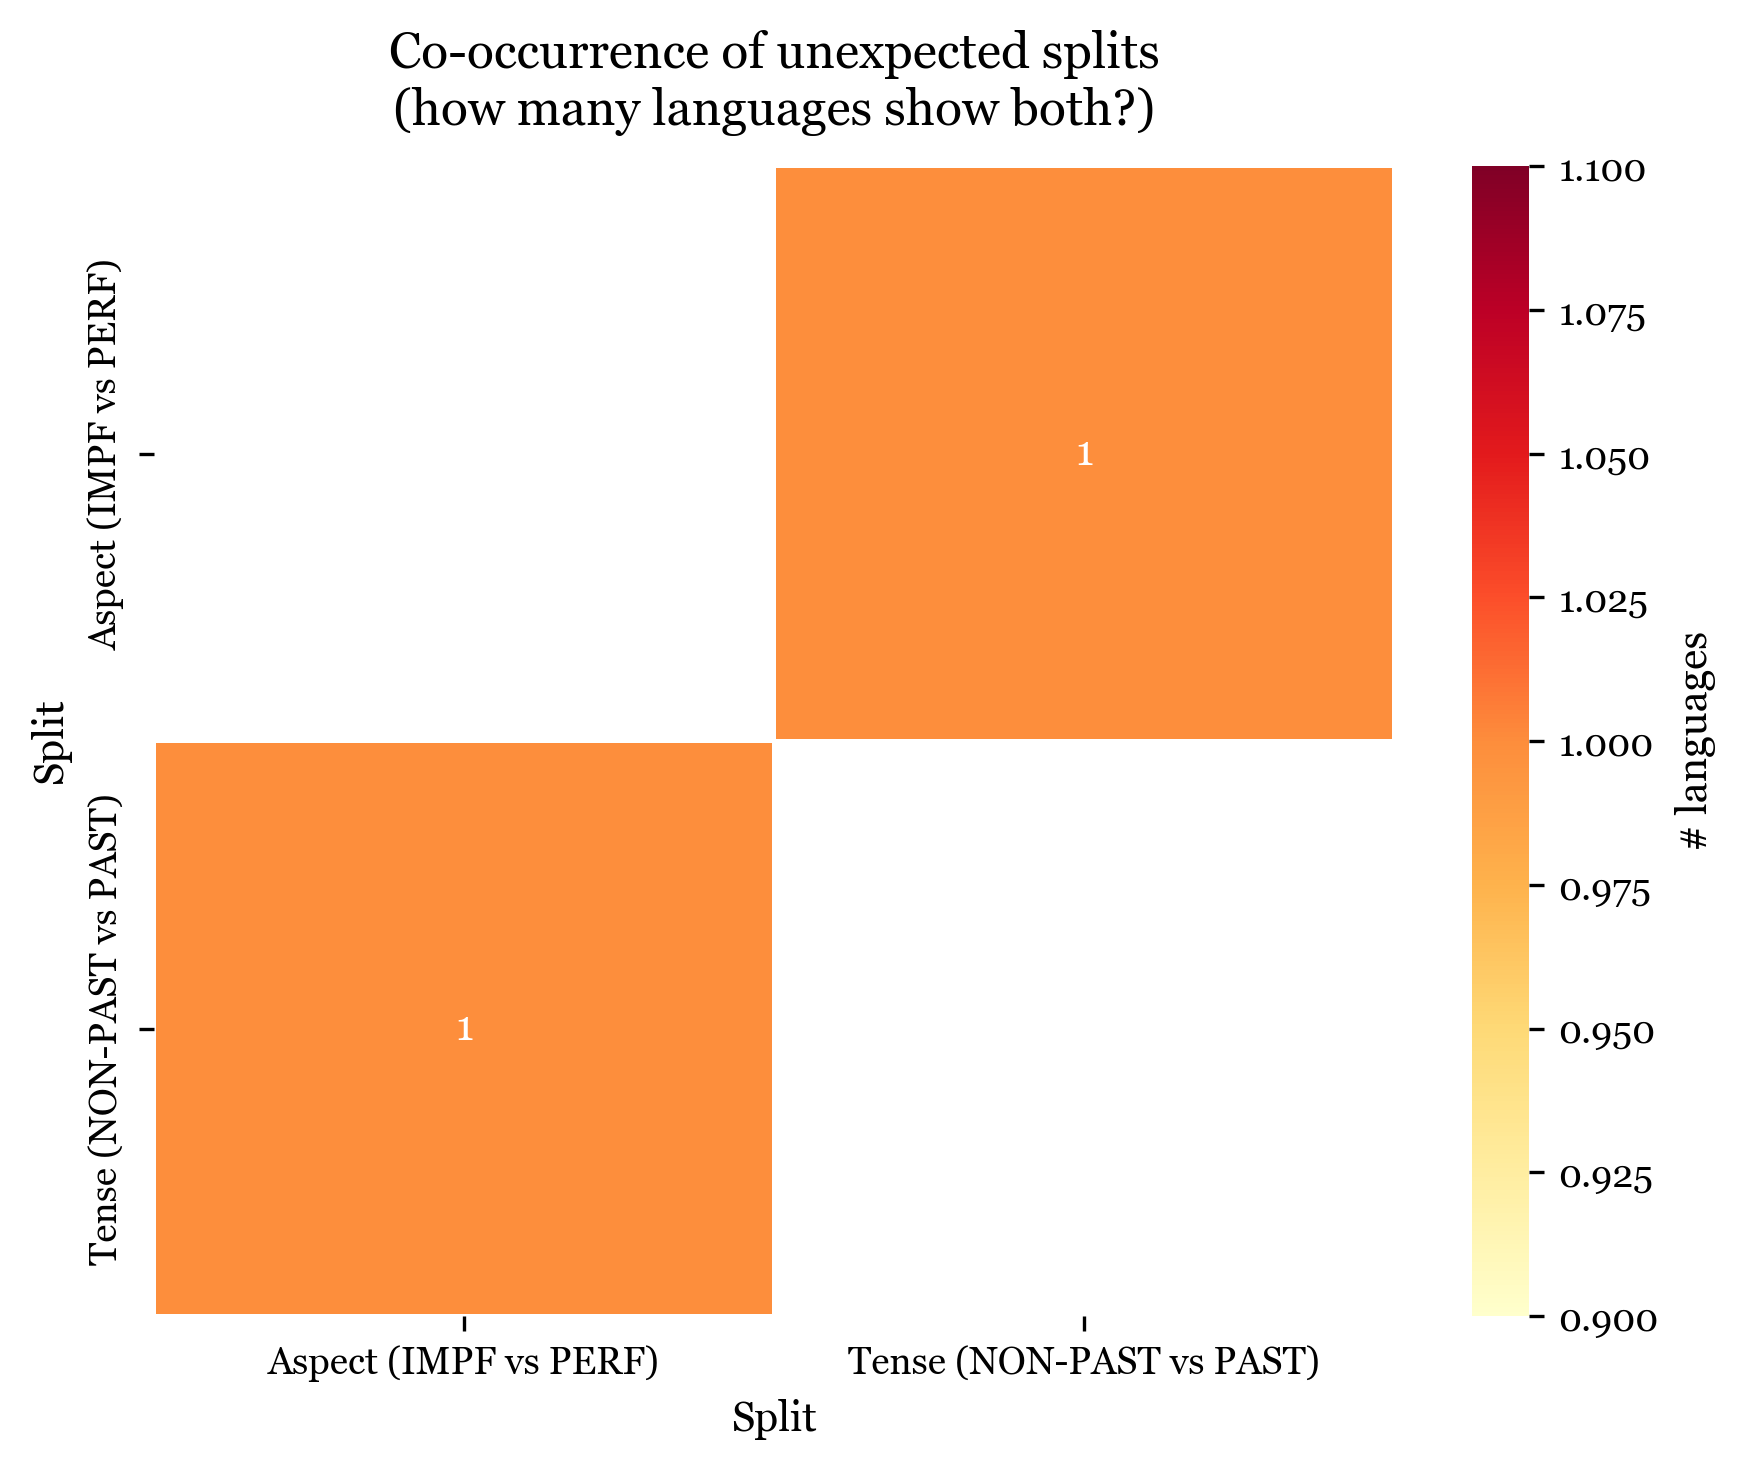
\includegraphics[width=0.55\textwidth]{figures/fig10_split_cooccurrence.png}
  \caption{Co-occurrence matrix: number of languages showing unexpected splits
    in both domains simultaneously.}
  \label{fig:cooccurrence}
\end{figure}

% ══════════════════════════════════════════════════════════════════════════════
\section{Analysis 4: Pairwise Feature Correlations}

\subsection{Method}

We computed all 276 pairwise phi ($\varphi$) coefficients between the 24 binary
features, restricted to languages with data on both features in each pair. The
phi coefficient is equivalent to Pearson's $r$ for binary variables and ranges
from $-1$ to $+1$. We also computed directed implication strengths $P(B \mid A)$
for all 552 ordered pairs, where values near 1.0 indicate near-universal
implications.

\subsection{Results}

Feature correlations are extraordinarily high within the tense/aspect/mood/realis
cluster. The ten strongest pairwise associations are shown in
Table~\ref{tab:phi}. The strongest associations are: perfective $\leftrightarrow$
past ($\varphi = 0.973$), indicative $\leftrightarrow$ realis ($\varphi =
0.972$), and past $\leftrightarrow$ indicative ($\varphi = 0.972$). These
near-perfect correlations indicate that languages that mark the ergative in the
past also mark it in the indicative and realis --- these are not independent
conditioning environments but a single coherent semantic cluster.

\begin{table}[H]
\centering
\caption{Top ten pairwise phi coefficients among the 24 ERGON features.}
\label{tab:phi}
\begin{tabular}{llrc}
\toprule
Feature A & Feature B & $\varphi$ & $n$ \\
\midrule
ERG: perfective     & ERG: past          & 0.973 & 171 \\
ERG: indicative     & ERG: realis        & 0.972 & 179 \\
ERG: past           & ERG: indicative    & 0.972 & 178 \\
ERG: perfective     & ERG: indicative    & 0.945 & 170 \\
ERG: non-indicative & ERG: irrealis      & 0.927 & 132 \\
ERG: past           & ERG: realis        & 0.918 & 177 \\
ERG: perfective     & ERG: animate A     & 0.917 & 171 \\
ERG: perfective     & ERG: realis        & 0.917 & 170 \\
ERG: 1st person     & ERG: 2nd person    & 0.914 & 178 \\
ERG: indicative     & ERG: animate A     & 0.914 & 177 \\
\bottomrule
\end{tabular}
\end{table}

A second tight cluster involves person features: 1st $\leftrightarrow$ 2nd
person ($\varphi = 0.914$). Several near-perfect implications ($P = 1.0$) were
identified: whenever a language marks the ergative in the non-indicative, it
invariably also marks it in the indicative; whenever it marks it in the realis,
it marks it in the indicative. The absolutive marker (GB409\_1) correlates weakly
or negatively with most conditioning features, suggesting it co-occurs with
simpler, less-conditioned ergativity systems.

\begin{figure}[H]
  \centering
  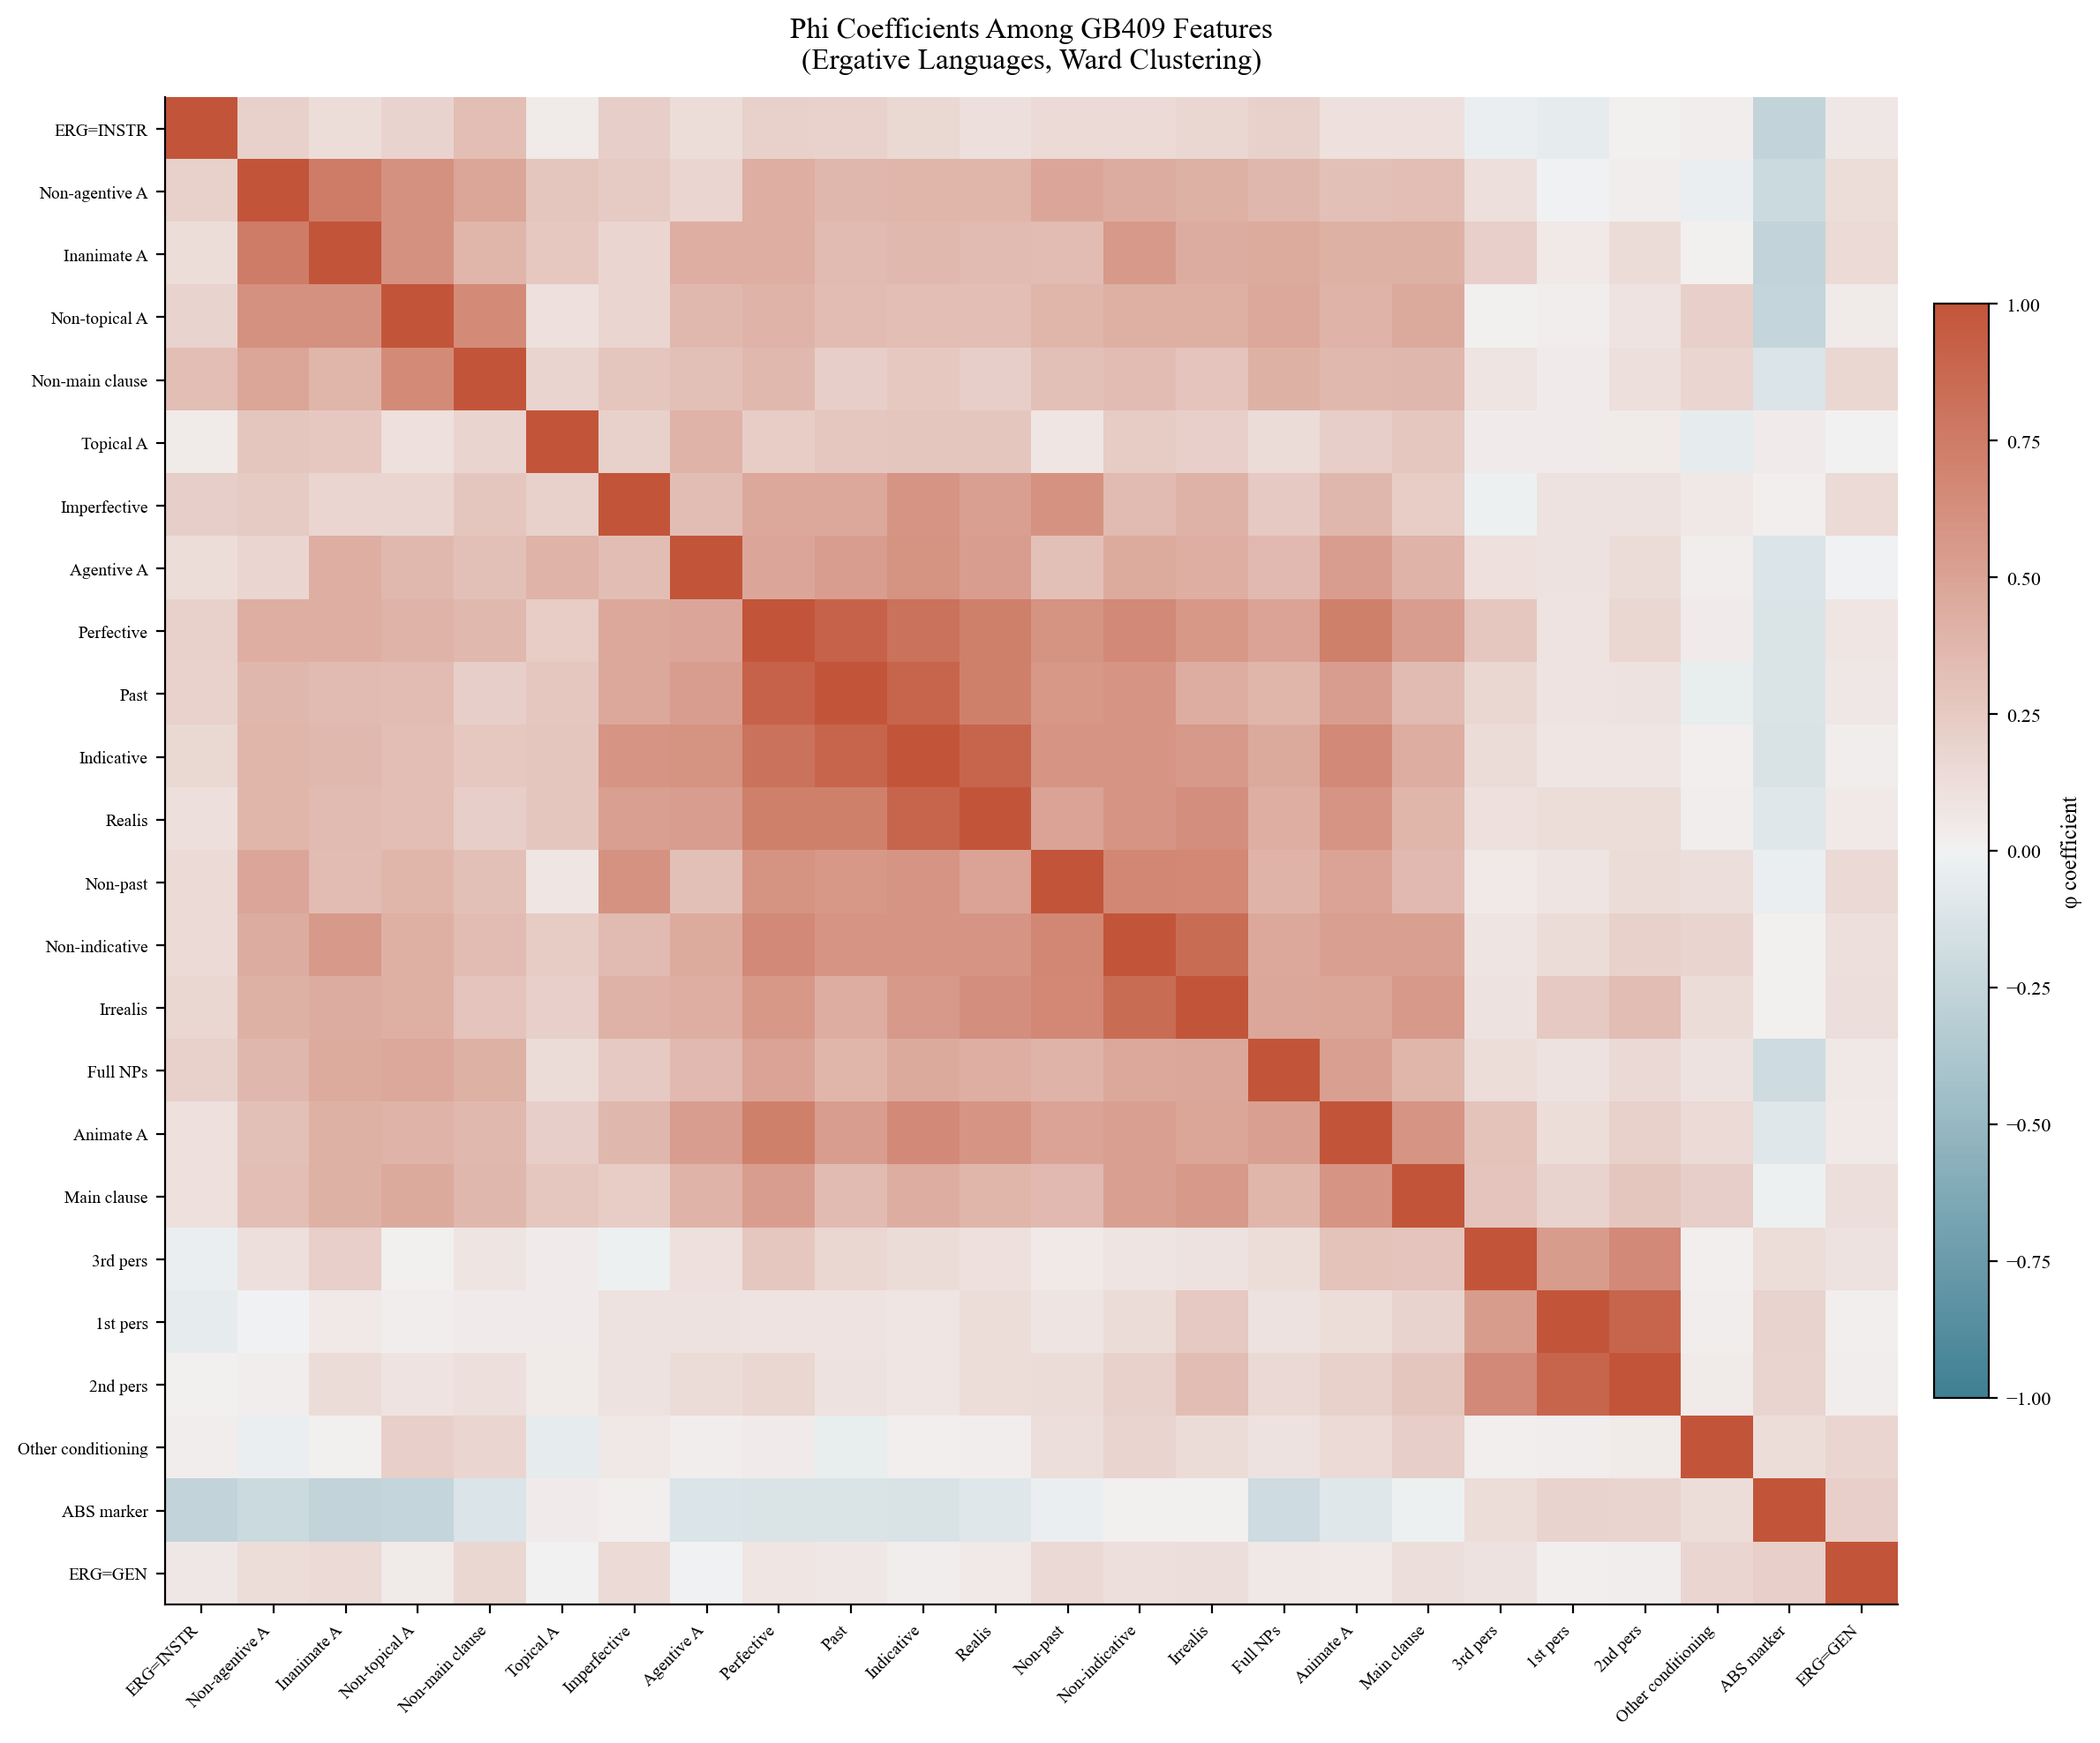
\includegraphics[width=0.88\textwidth]{figures/figA_phi_heatmap.png}
  \caption{Phi coefficient heatmap for all 276 feature pairs. Features are
    ordered by domain.}
  \label{fig:phi_heatmap}
\end{figure}

\begin{figure}[H]
  \centering
  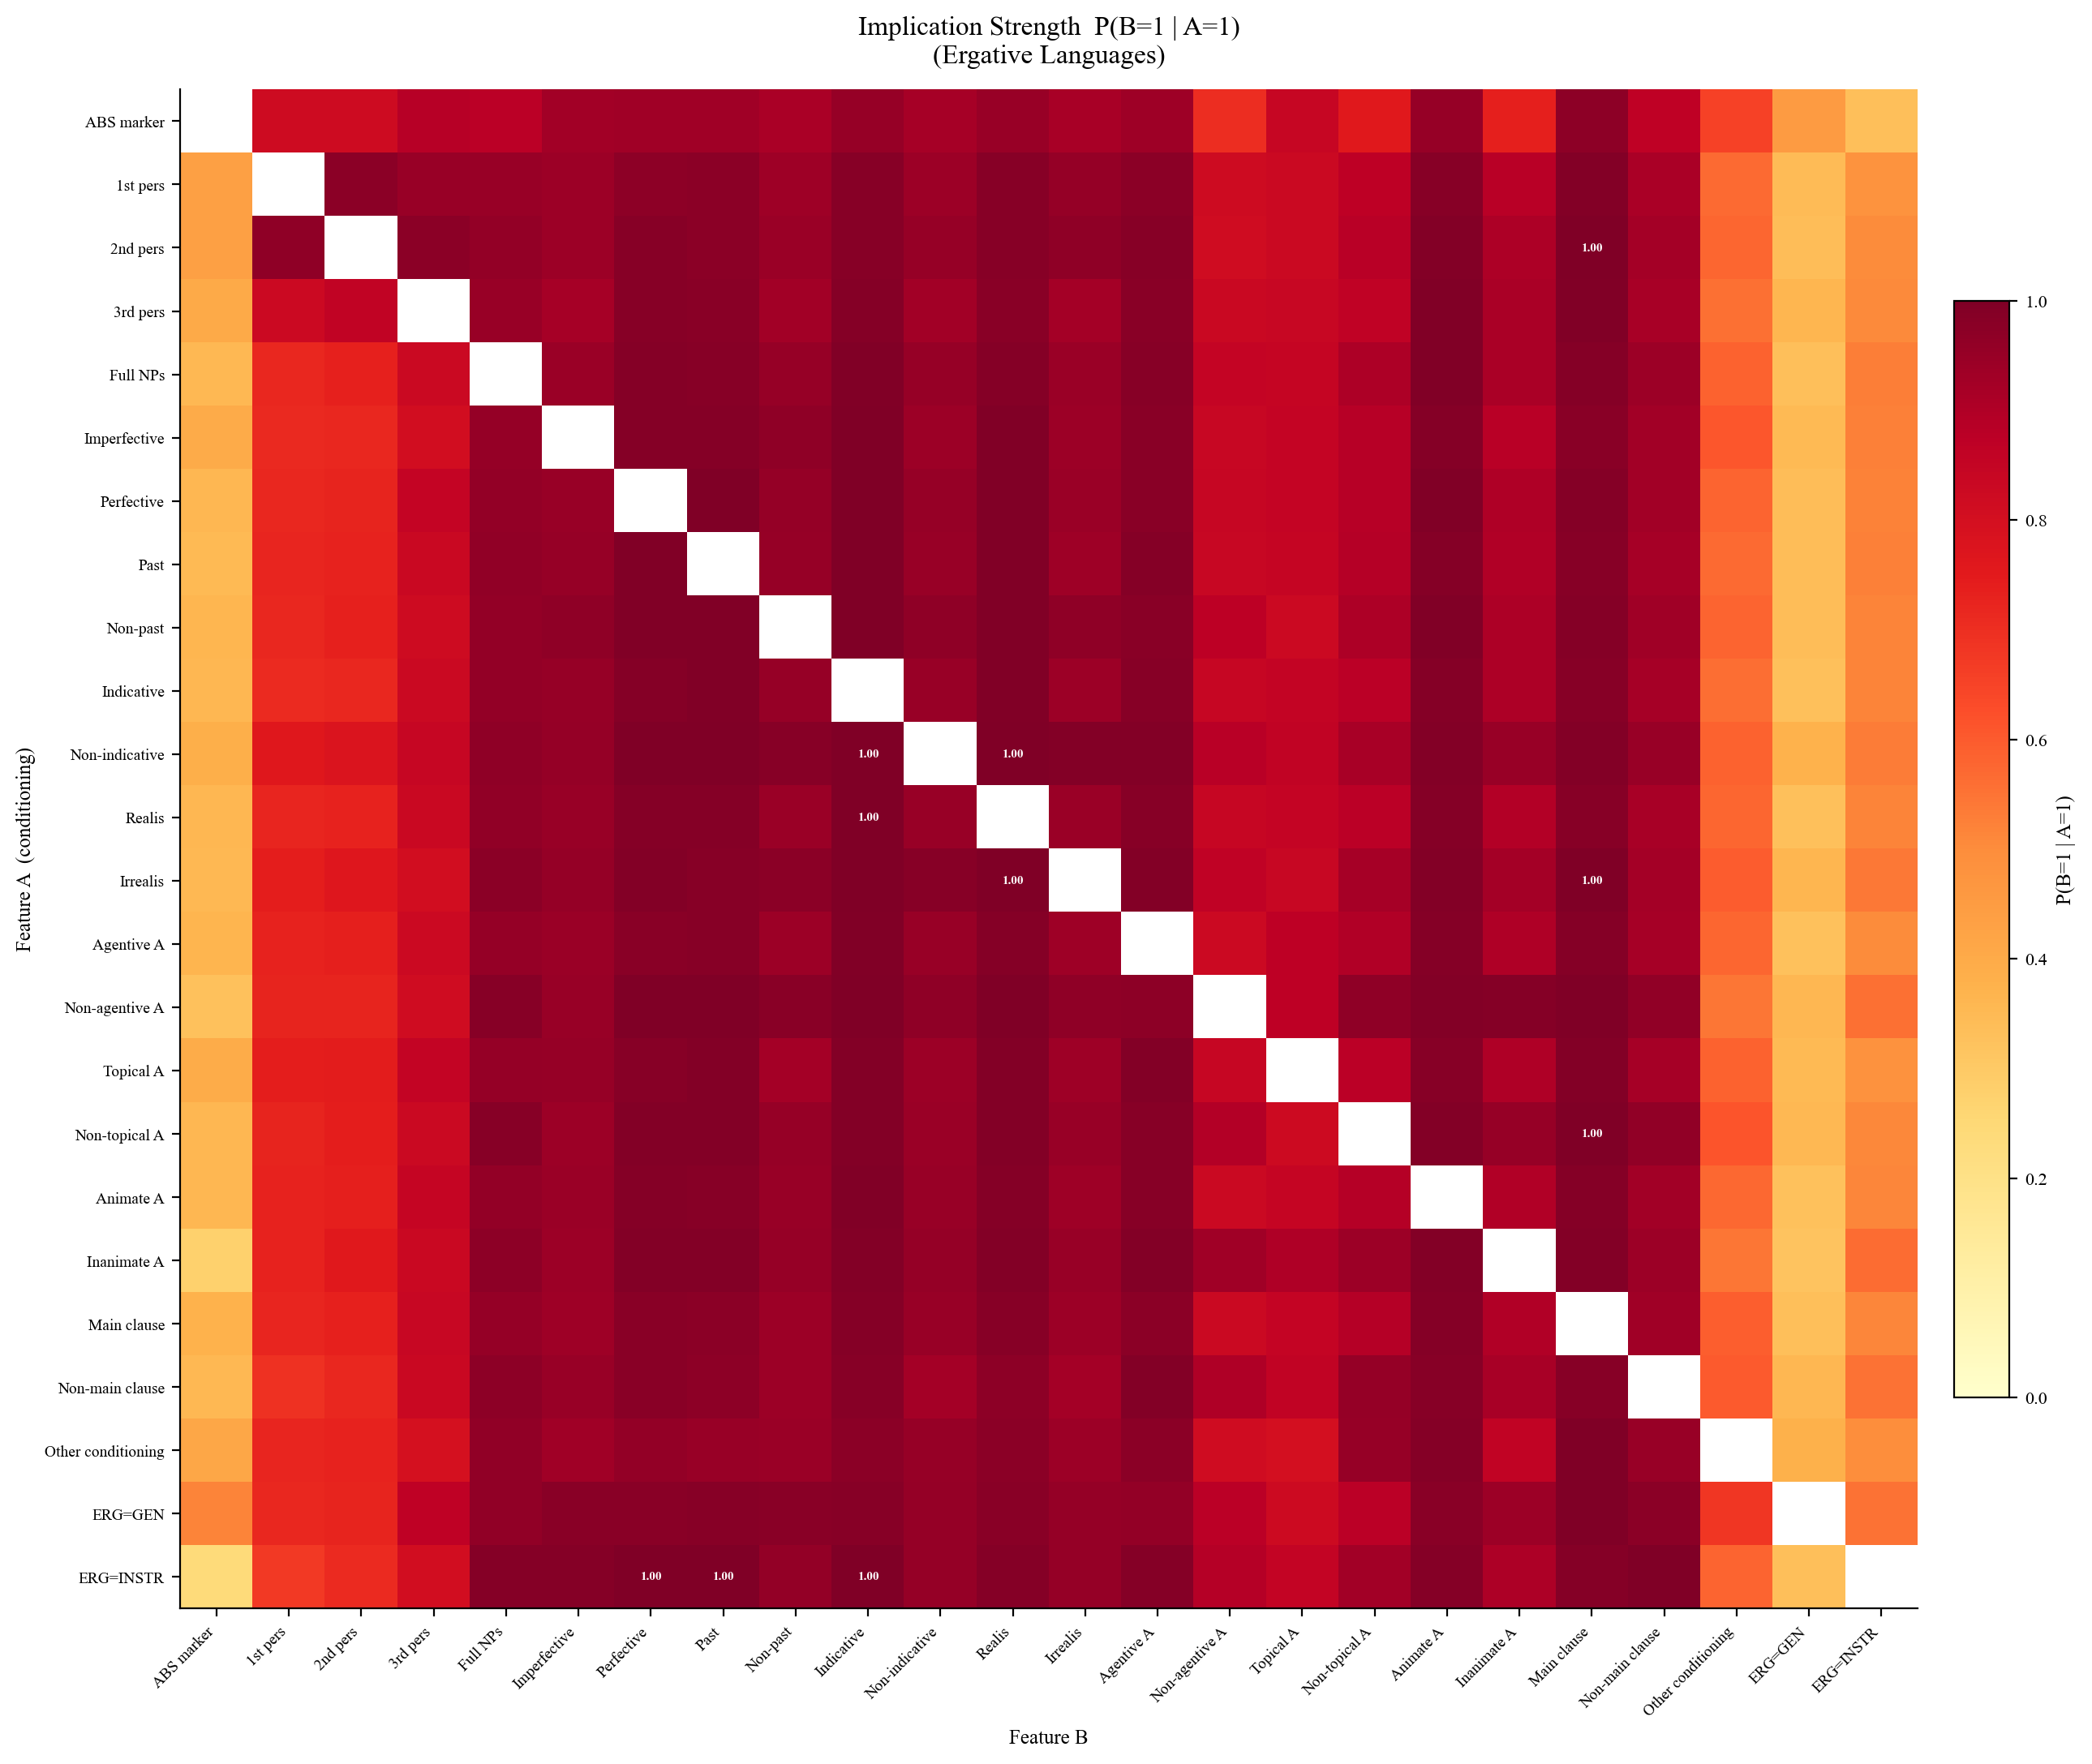
\includegraphics[width=0.88\textwidth]{figures/figB_implication_matrix.png}
  \caption{Directed implication matrix: $P(\text{column} \mid \text{row})$.
    Dark cells indicate near-universal implications.}
  \label{fig:implication}
\end{figure}

% ══════════════════════════════════════════════════════════════════════════════
\section{Analysis 5: Feature Predictors of Ergativity Score}

\subsection{Method}

To identify which individual features best predict overall ergativity score, we
computed point-biserial correlations between each binary feature and the
continuous ergativity score from Analysis~1. Point-biserial $r$ is equivalent to
Pearson's $r$ when one variable is binary. Significance was assessed using
$t$-tests with Bonferroni correction for 24 comparisons (adjusted
$\alpha = 0.002$).

\subsection{Results}

All 24 features are significantly correlated with ergativity score after
Bonferroni correction. The strongest predictors are from the
tense/aspect/mood/realis cluster: perfective ($r = +0.919$), indicative
($r = +0.917$), animate A ($r = +0.905$), realis ($r = +0.903$), and past
($r = +0.892$). A single feature from this cluster can predict nearly 80\% of
variance in total ergativity score.

The weakest --- though still significant --- predictors are: absolutive marker
($r = +0.237$), ergative~=~genitive ($r = +0.243$), other conditioning
($r = +0.278$), and ergative~=~instrumental ($r = +0.317$). Whether the ergative
marker is formally identical to the genitive or instrumental is a morphological
accident largely independent of how systematically ergative alignment is deployed
across domains.

\begin{figure}[H]
  \centering
  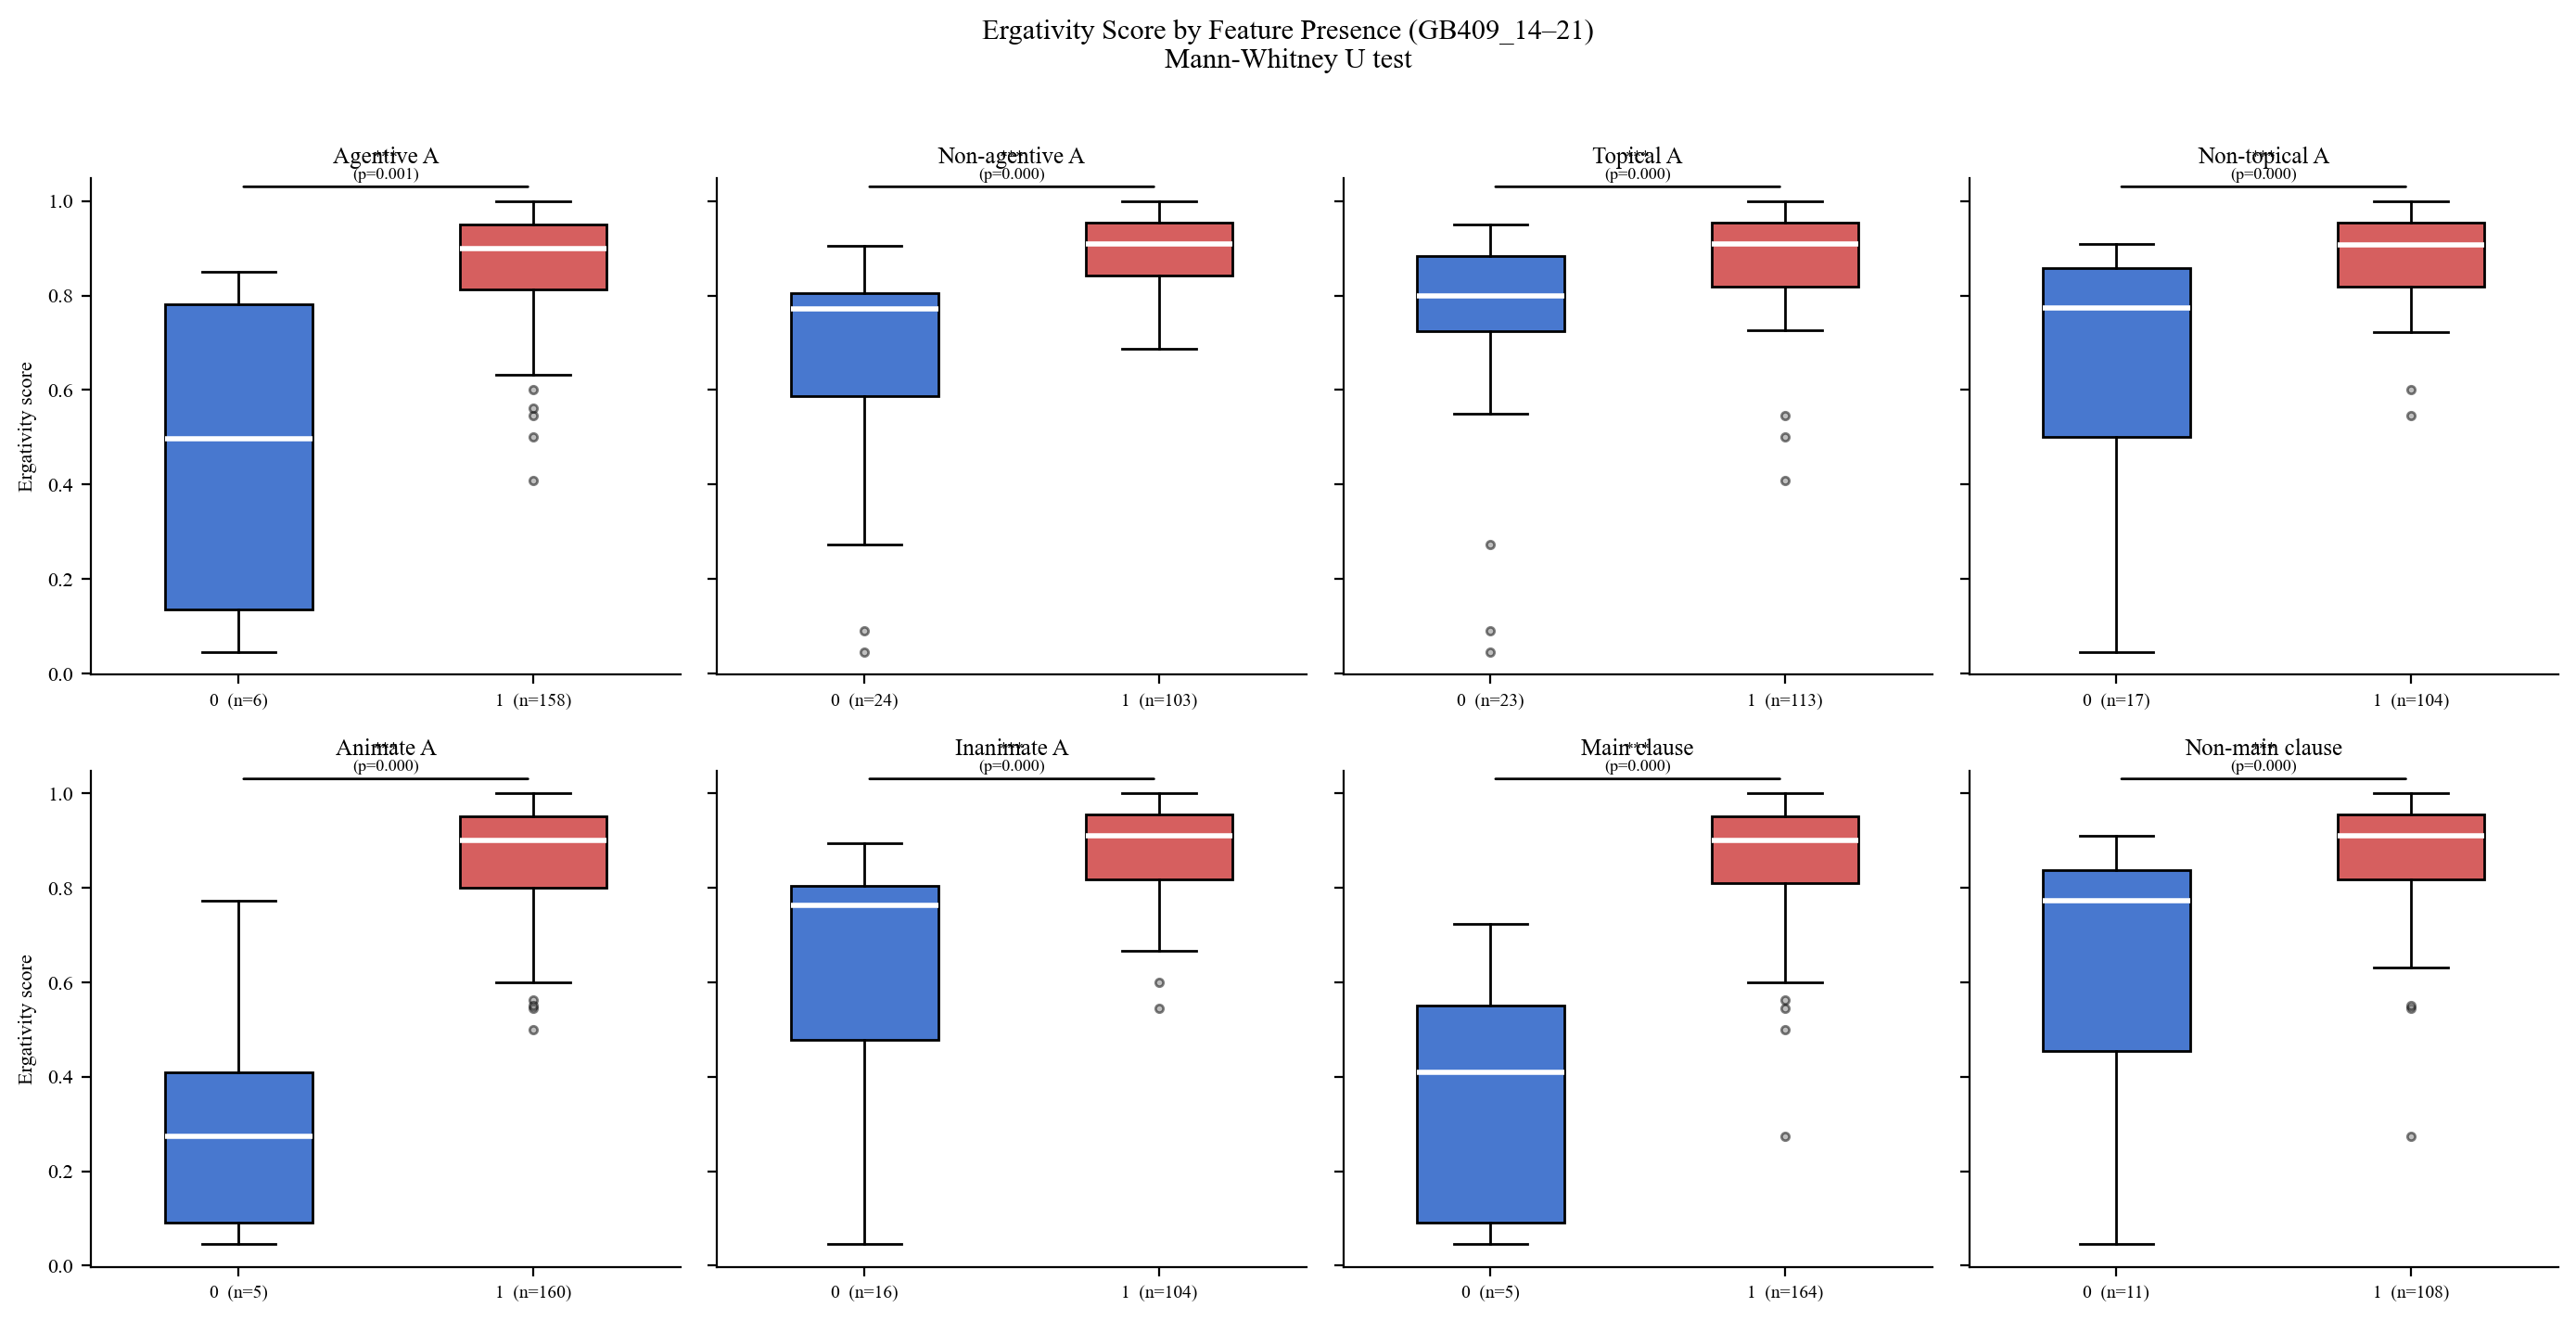
\includegraphics[width=0.88\textwidth]{figures/figA_boxplots.png}
  \caption{Ergativity score distributions split by feature value (0/1) for the
    8 strongest predictors.}
  \label{fig:boxplots}
\end{figure}

\begin{figure}[H]
  \centering
  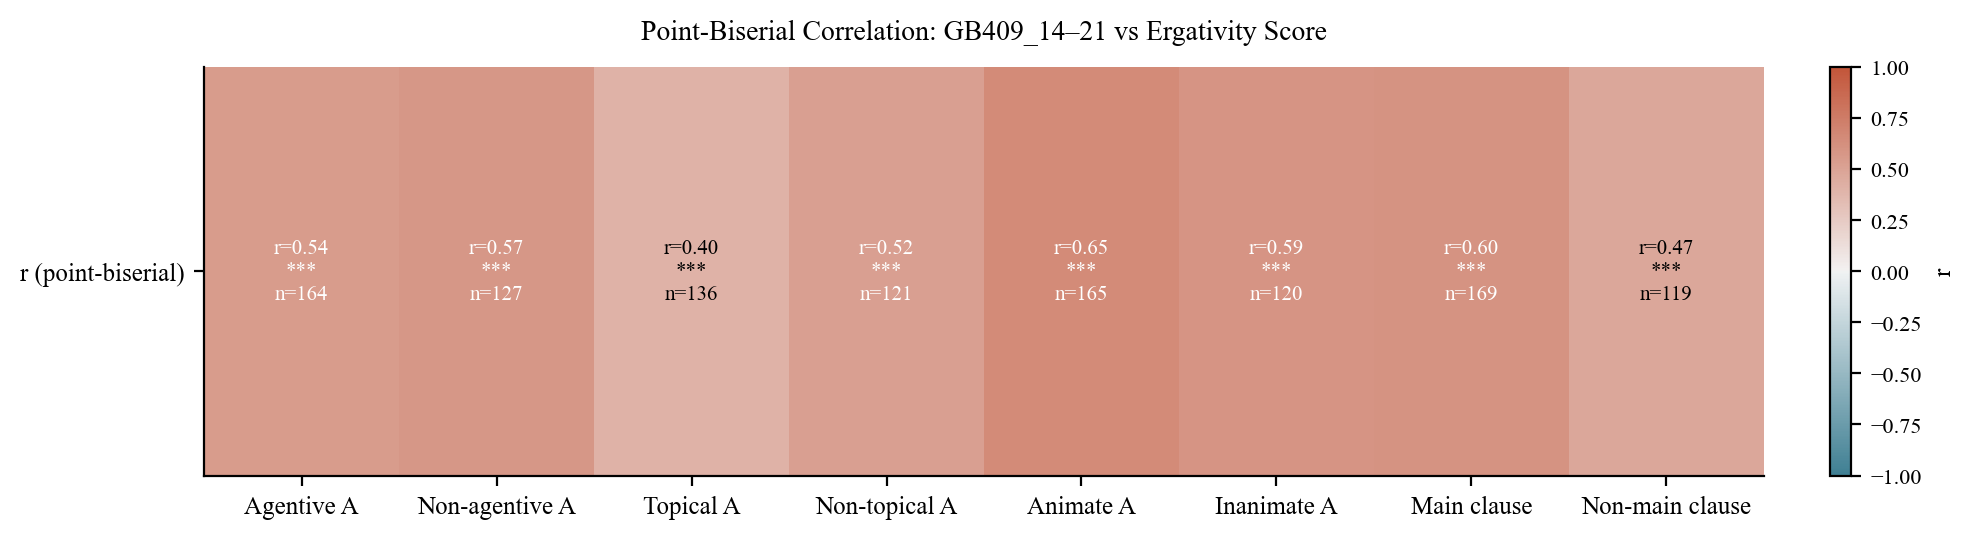
\includegraphics[width=0.82\textwidth]{figures/figB_pointbiserial.png}
  \caption{Point-biserial correlations between each feature and ergativity score,
    with 95\% confidence intervals. All values are statistically significant after
    Bonferroni correction.}
  \label{fig:pointbiserial}
\end{figure}

\begin{figure}[H]
  \centering
  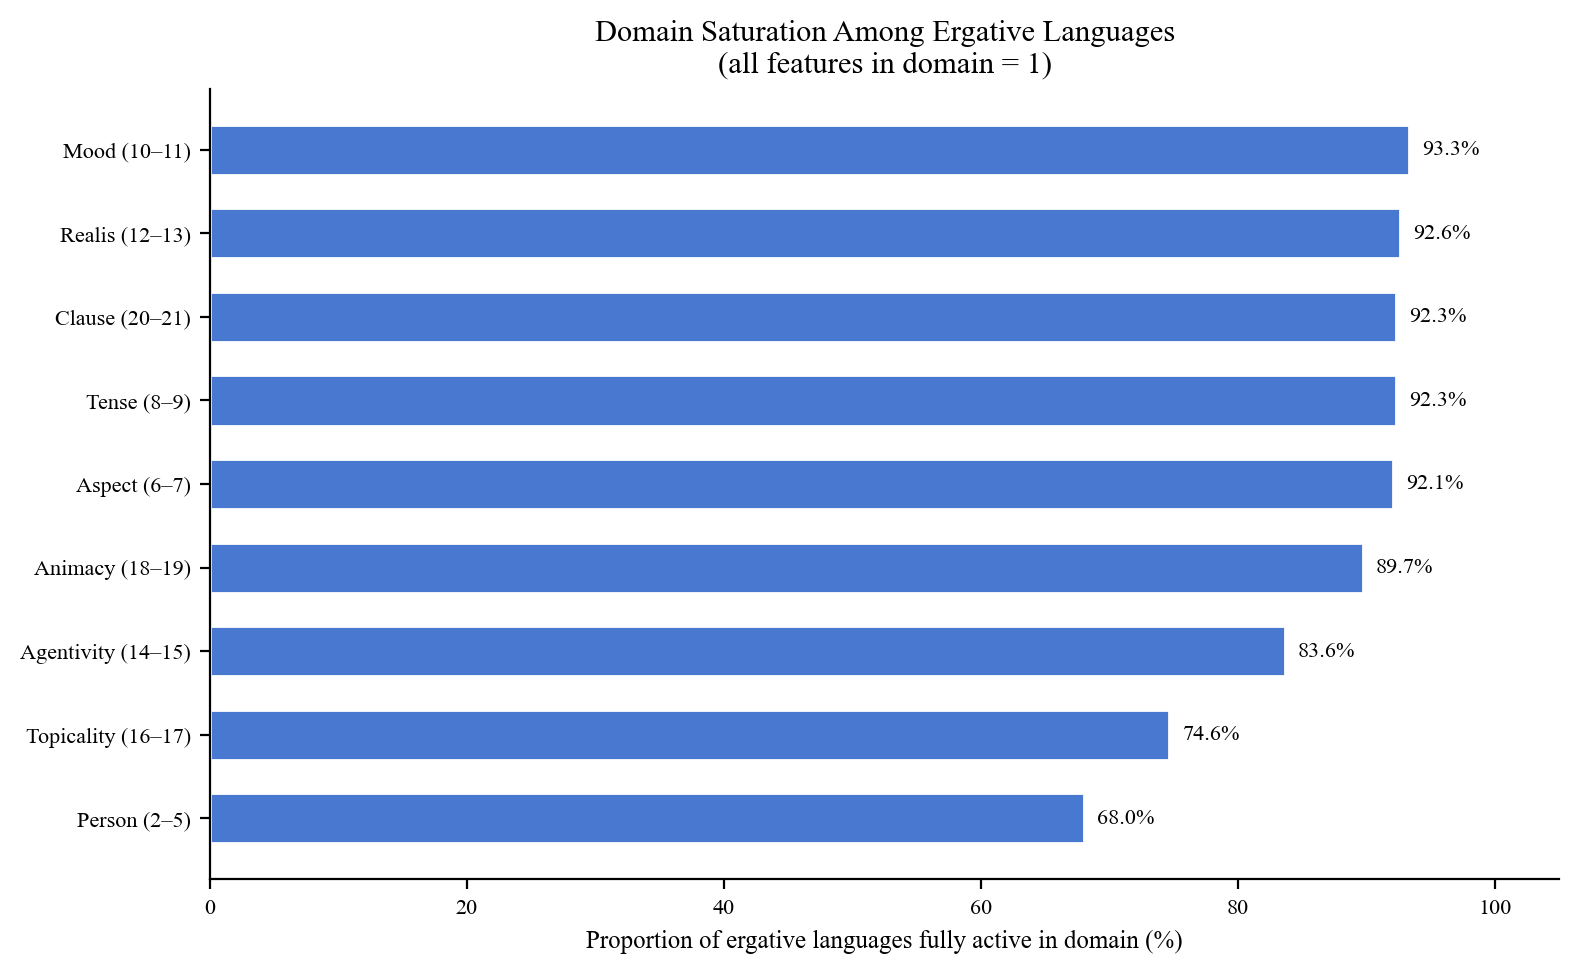
\includegraphics[width=0.72\textwidth]{figures/figC_domain_activity.png}
  \caption{Mean ergativity score by conditioning domain.}
  \label{fig:domain_activity}
\end{figure}

% ══════════════════════════════════════════════════════════════════════════════
\section{Analysis 6: Ergativity Dimensionality Index}

\subsection{Method}

Beyond a total score, we asked: in how many distinct conditioning domains does a
language deploy ergative marking? We defined nine domains --- Person
(GB409\_2--5), Aspect (6--7), Tense (8--9), Mood (10--11), Realis (12--13),
Agentivity (14--15), Topicality (16--17), Animacy (18--19), and Clause type
(20--21) --- and classified each domain per language as: \textit{full} (both
features~= 1), \textit{partial} (mixed), or \textit{absent} (both~= 0 or no
data). The dimensionality index equals the number of fully active domains
(range 0--9).

\subsection{Results}

Among 180 ergative languages, the mean dimensionality is 7.30 ($SD = 2.06$),
ranging from 0 to 9. Most languages deploy ergative marking broadly: Clause type
is the most universally active domain (91.7\% of languages fully active), followed
by Tense (89.4\%) and Mood (88.9\%). Topicality is the least commonly active
(57.8\%), reflecting the relative rarity of topicality-conditioned ergativity
splits.

\begin{table}[H]
\centering
\caption{Domain coverage rates across 180 ergative languages.}
\label{tab:domains}
\begin{tabular}{lrr}
\toprule
Domain & Full (\%) & Partial (\%) \\
\midrule
Clause type  & 91.7 &  5.6 \\
Tense        & 89.4 &  4.4 \\
Mood         & 88.9 &  3.9 \\
Realis       & 86.7 &  3.9 \\
Animacy      & 85.0 &  7.2 \\
Aspect       & 84.4 &  5.0 \\
Agentivity   & 78.9 & 13.3 \\
Person       & 67.2 & 31.7 \\
Topicality   & 57.8 & 16.7 \\
\bottomrule
\end{tabular}
\end{table}

Trans-Himalayan languages show the highest mean dimensionality among
well-represented families, while Austronesian and Indo-European languages show
lower and more variable dimensionality indices. The Person domain is unique in
having substantial partial coverage (31.7\%), corresponding to languages that mark
ergative on some but not all person categories --- consistent with the Silverstein
gradient.

\begin{figure}[H]
  \centering
  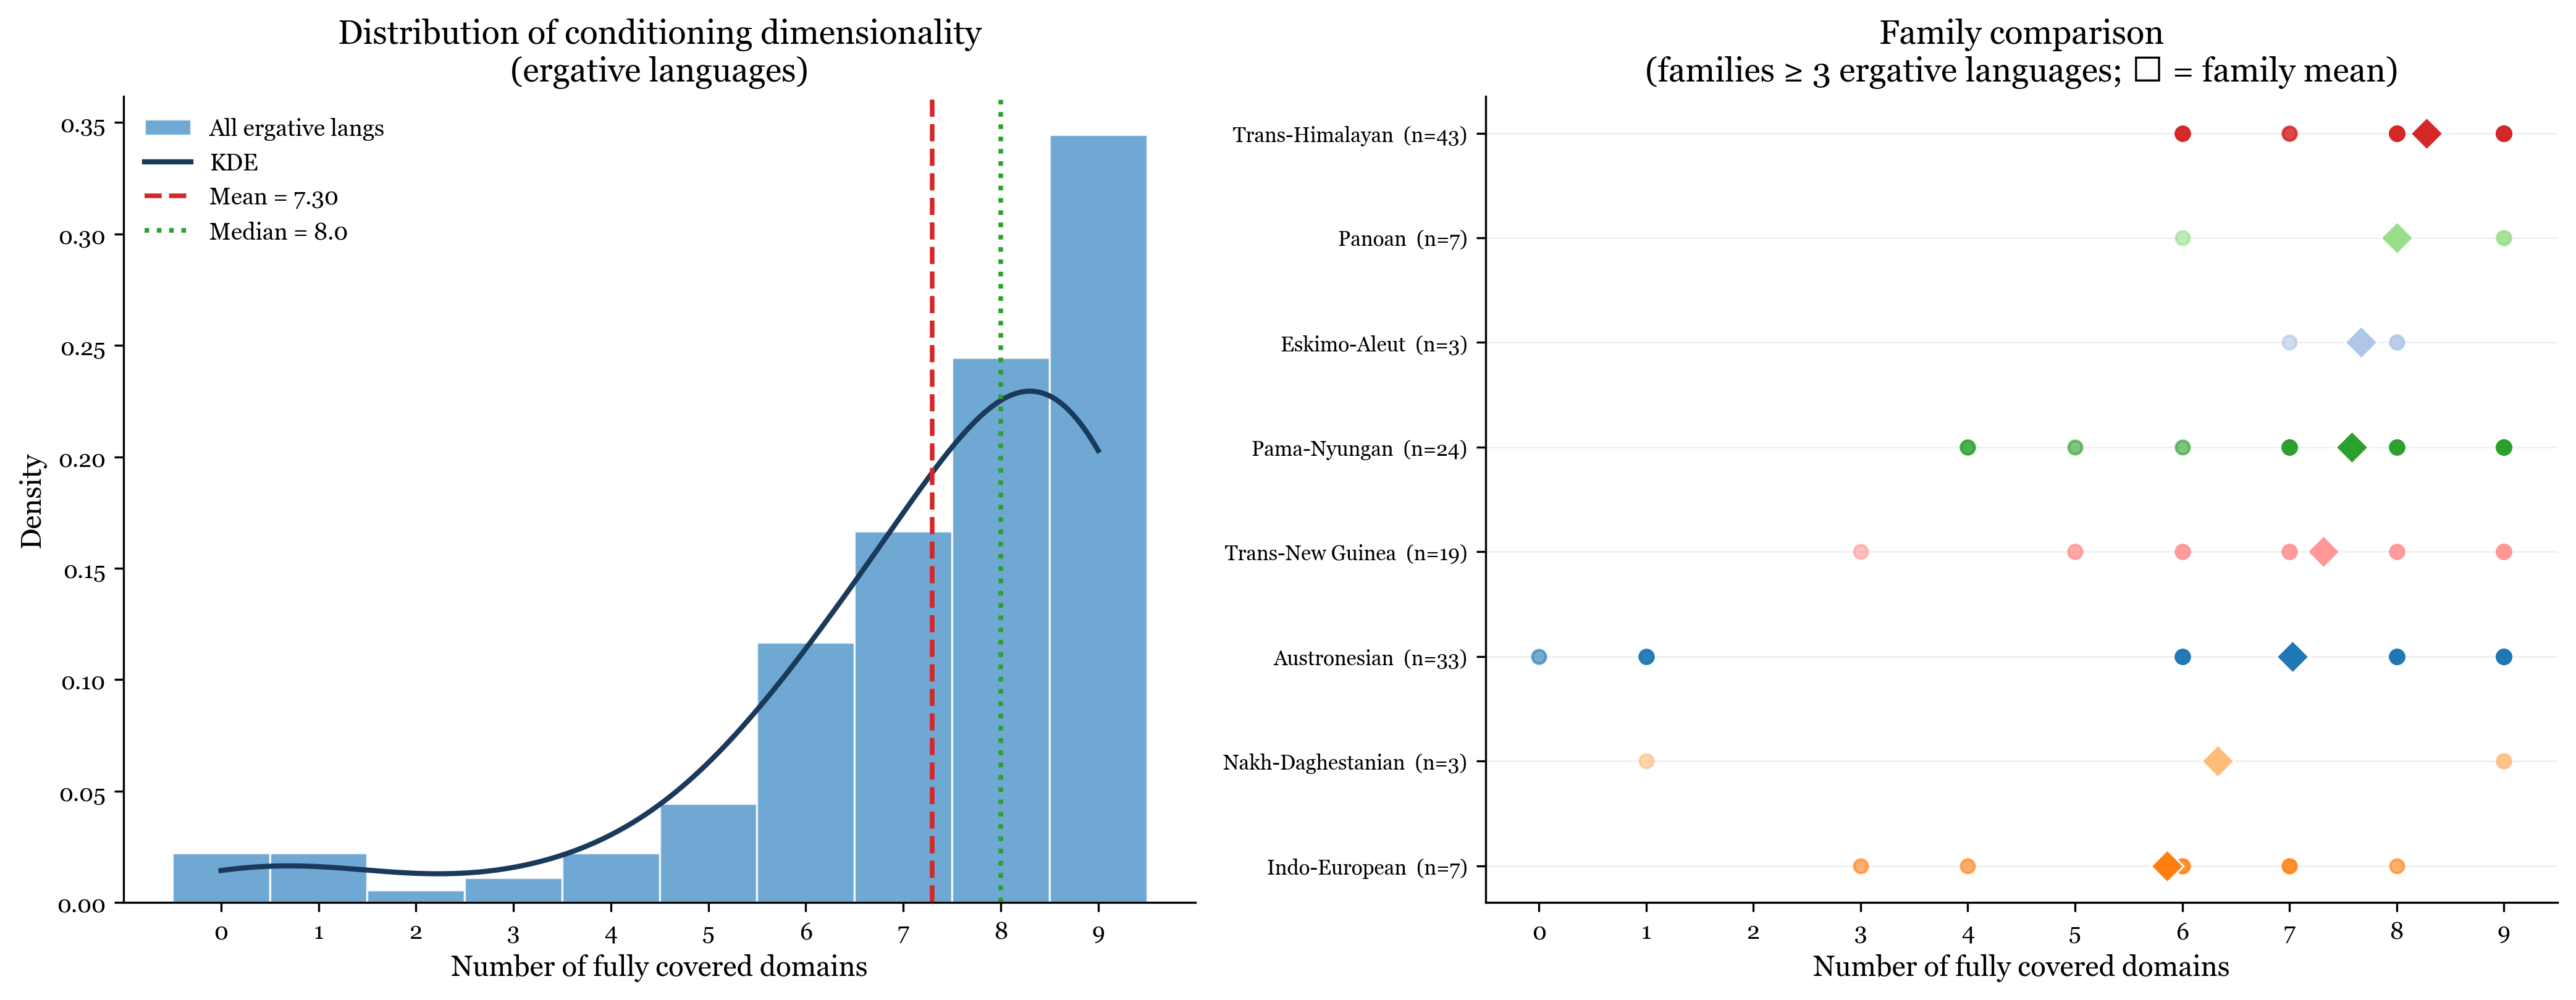
\includegraphics[width=0.82\textwidth]{figures/figA_dimensionality_distribution.png}
  \caption{Distribution of the ergativity dimensionality index across ergative
    languages.}
  \label{fig:dim_dist}
\end{figure}

\begin{figure}[H]
  \centering
  
\includegraphics[width=0.92\textwidth]{figures/figB_dimensionality_heatmap.png}
  \caption{Domain activity heatmap. Dark~= fully active, medium~= partial,
    light~= absent.}
  \label{fig:dim_heatmap}
\end{figure}

\begin{figure}[H]
  \centering
  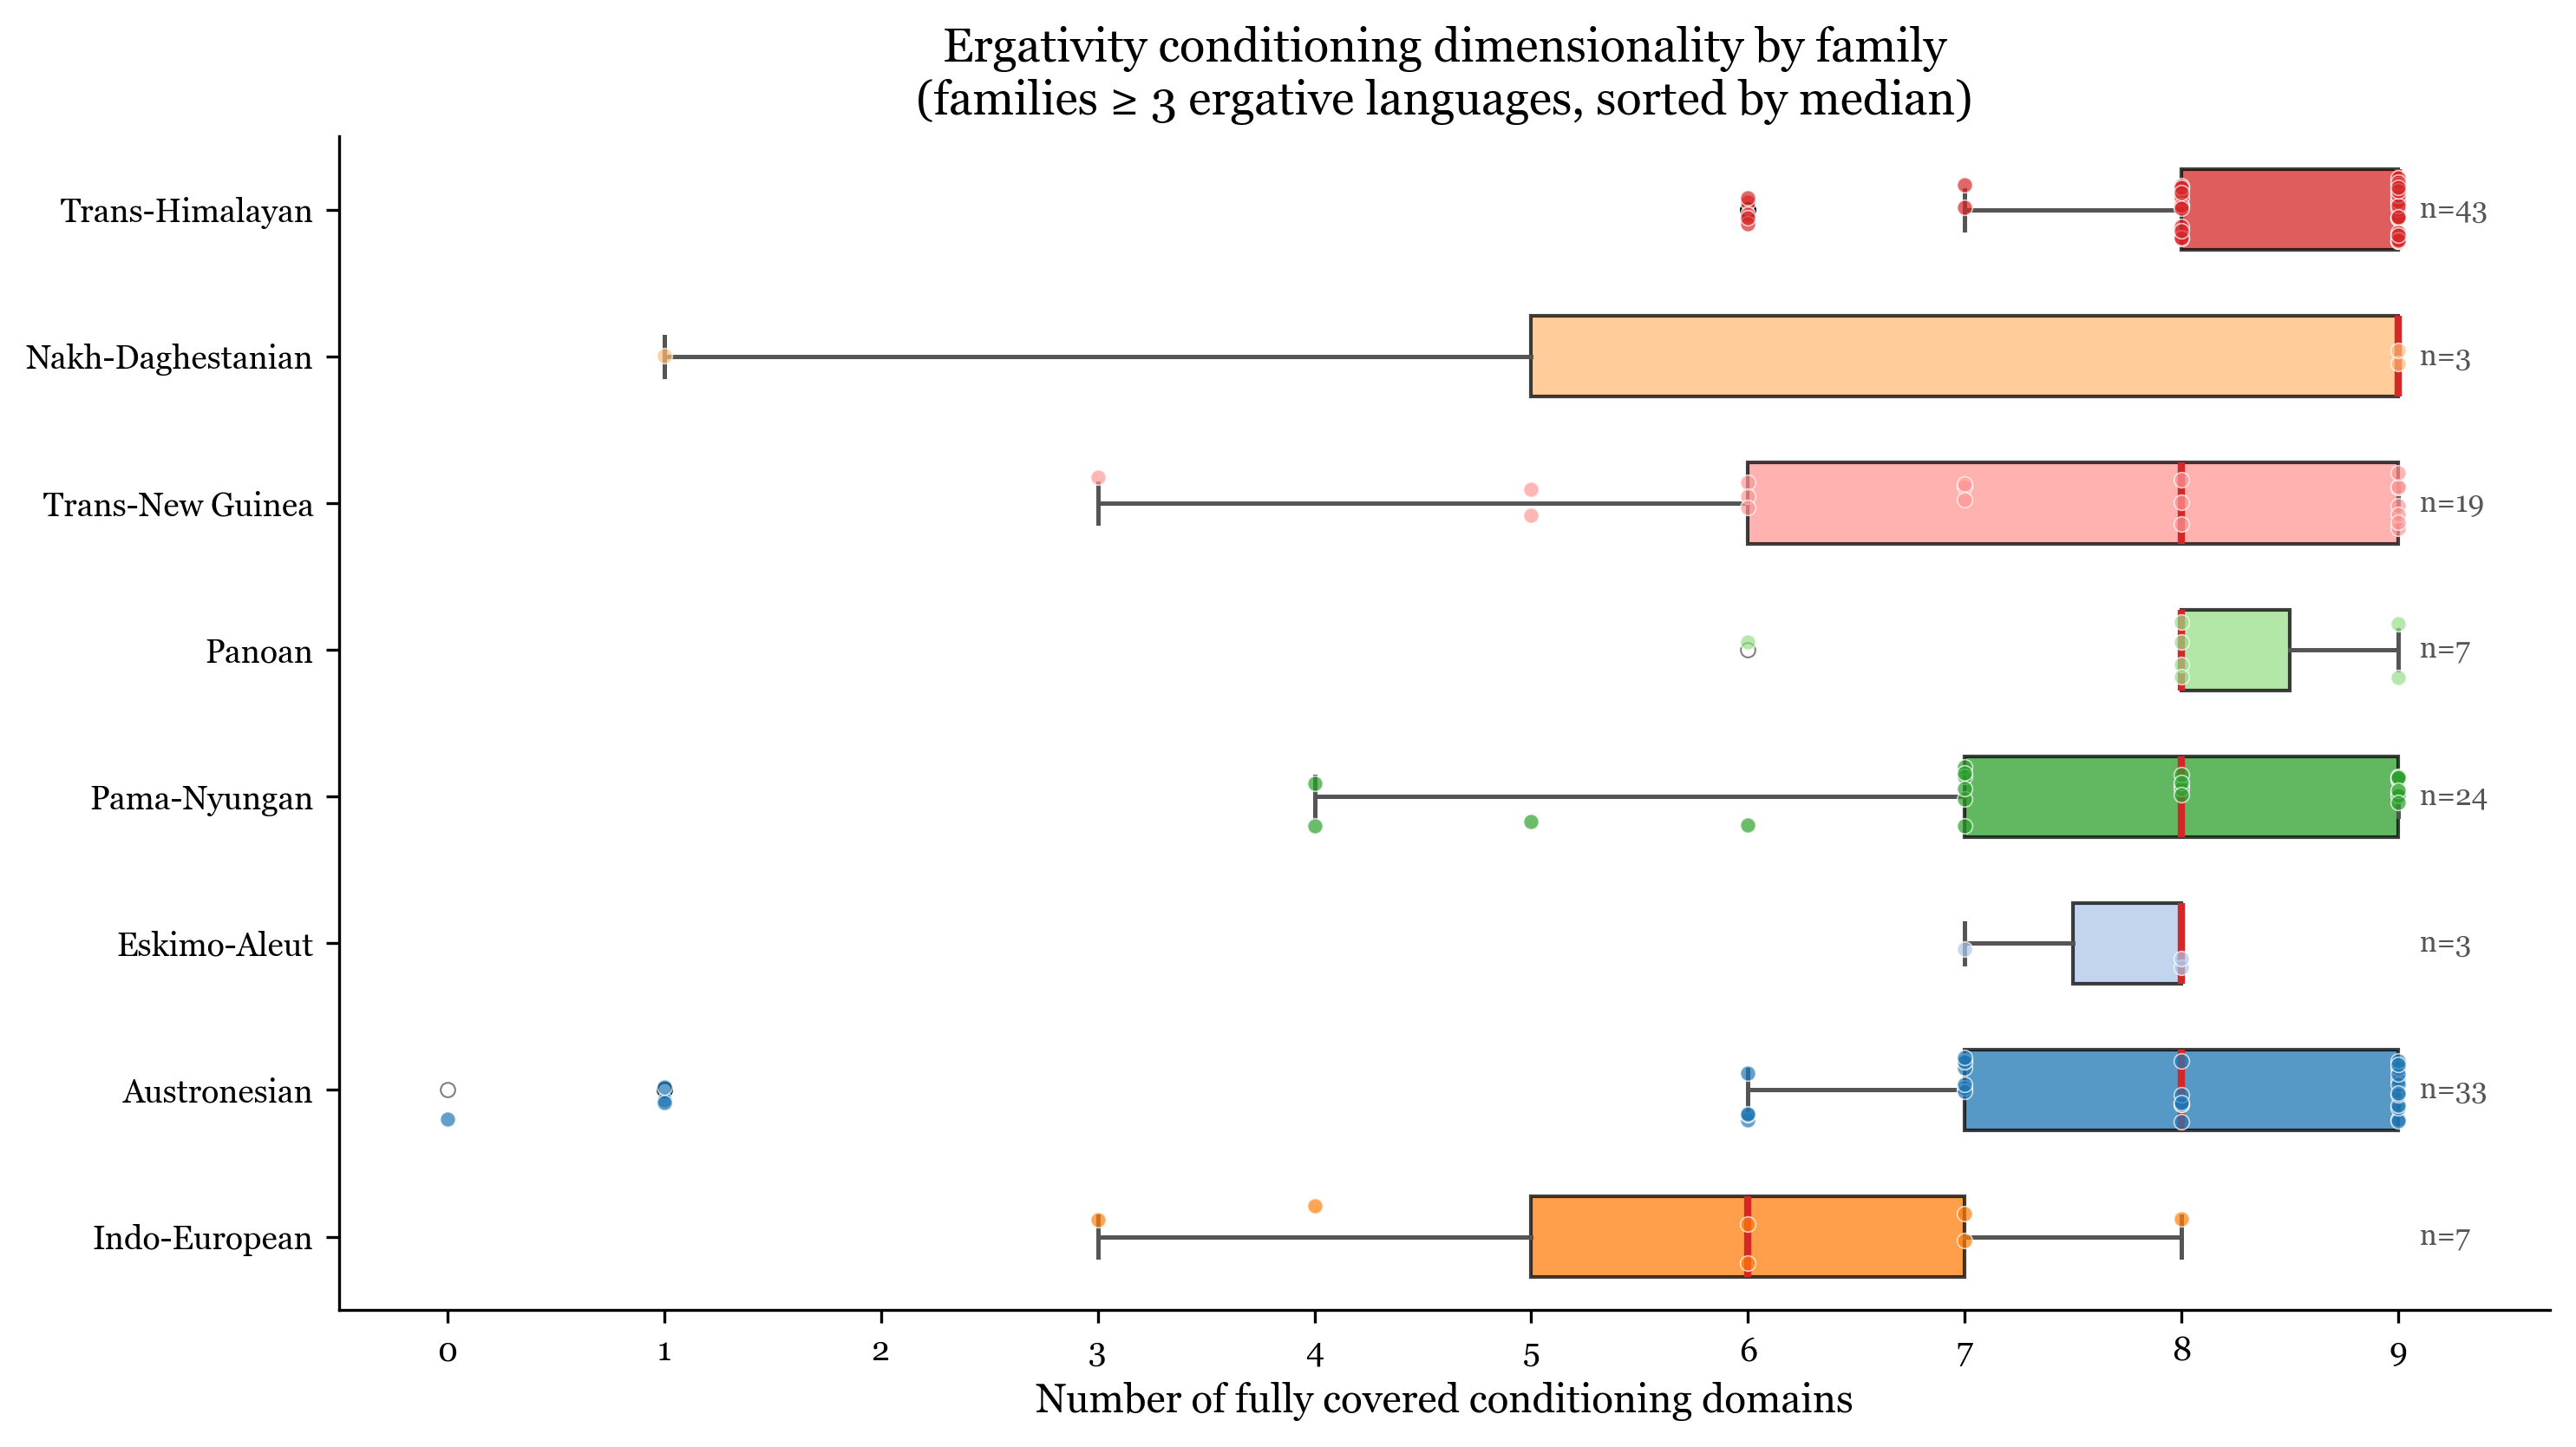
\includegraphics[width=0.82\textwidth]{figures/figC_dimensionality_boxplot.png}
  \caption{Dimensionality index by language family (families with $\geq 3$
    languages).}
  \label{fig:dim_boxplot}
\end{figure}

% ══════════════════════════════════════════════════════════════════════════════
\section{Analysis 7: Phylogenetic Signal}

\subsection{Method}

We estimated phylogenetic signal using two complementary approaches. First,
$\eta^2$ (eta-squared) measures variance in ergativity score explained by family
membership via one-way ANOVA across families with $\geq 3$ languages; significance
was assessed by permutation test (10,000 permutations). Second, Cram\'er's $V$
measures the association between each binary feature and family membership
(categorical), providing a per-feature phylogenetic conservatism index.

\subsection{Results}

Family membership explains $\eta^2 = 0.409$ of variance in ergativity scores ---
a large effect by conventional standards \citep{cohen1988}. The permutation test
yields $p = 0.059$ (marginally non-significant at $\alpha = 0.05$), reflecting
the tension between a substantial typological effect and limited power with few
independent genealogical units (families).

The most phylogenetically conserved features are ERG~=~GEN ($V = 0.655$),
imperfective ($V = 0.621$), and 2nd person ($V = 0.482$) --- strongly
family-specific properties largely inherited rather than convergently acquired.
The least conserved are main clause ($V = 0.157$), realis ($V = 0.167$), and
indicative ($V = 0.227$), suggesting these are more susceptible to independent
development or loss.

Among families, Eskimo-Aleut ($CV = 0.028$) and Indo-European ($CV = 0.060$) are
the most internally consistent. Nakh-Daghestanian ($CV = 0.327$) and Austronesian
($CV = 0.235$) show the greatest internal heterogeneity, reflecting the
well-known typological diversity within these large families.

\begin{figure}[H]
  \centering
  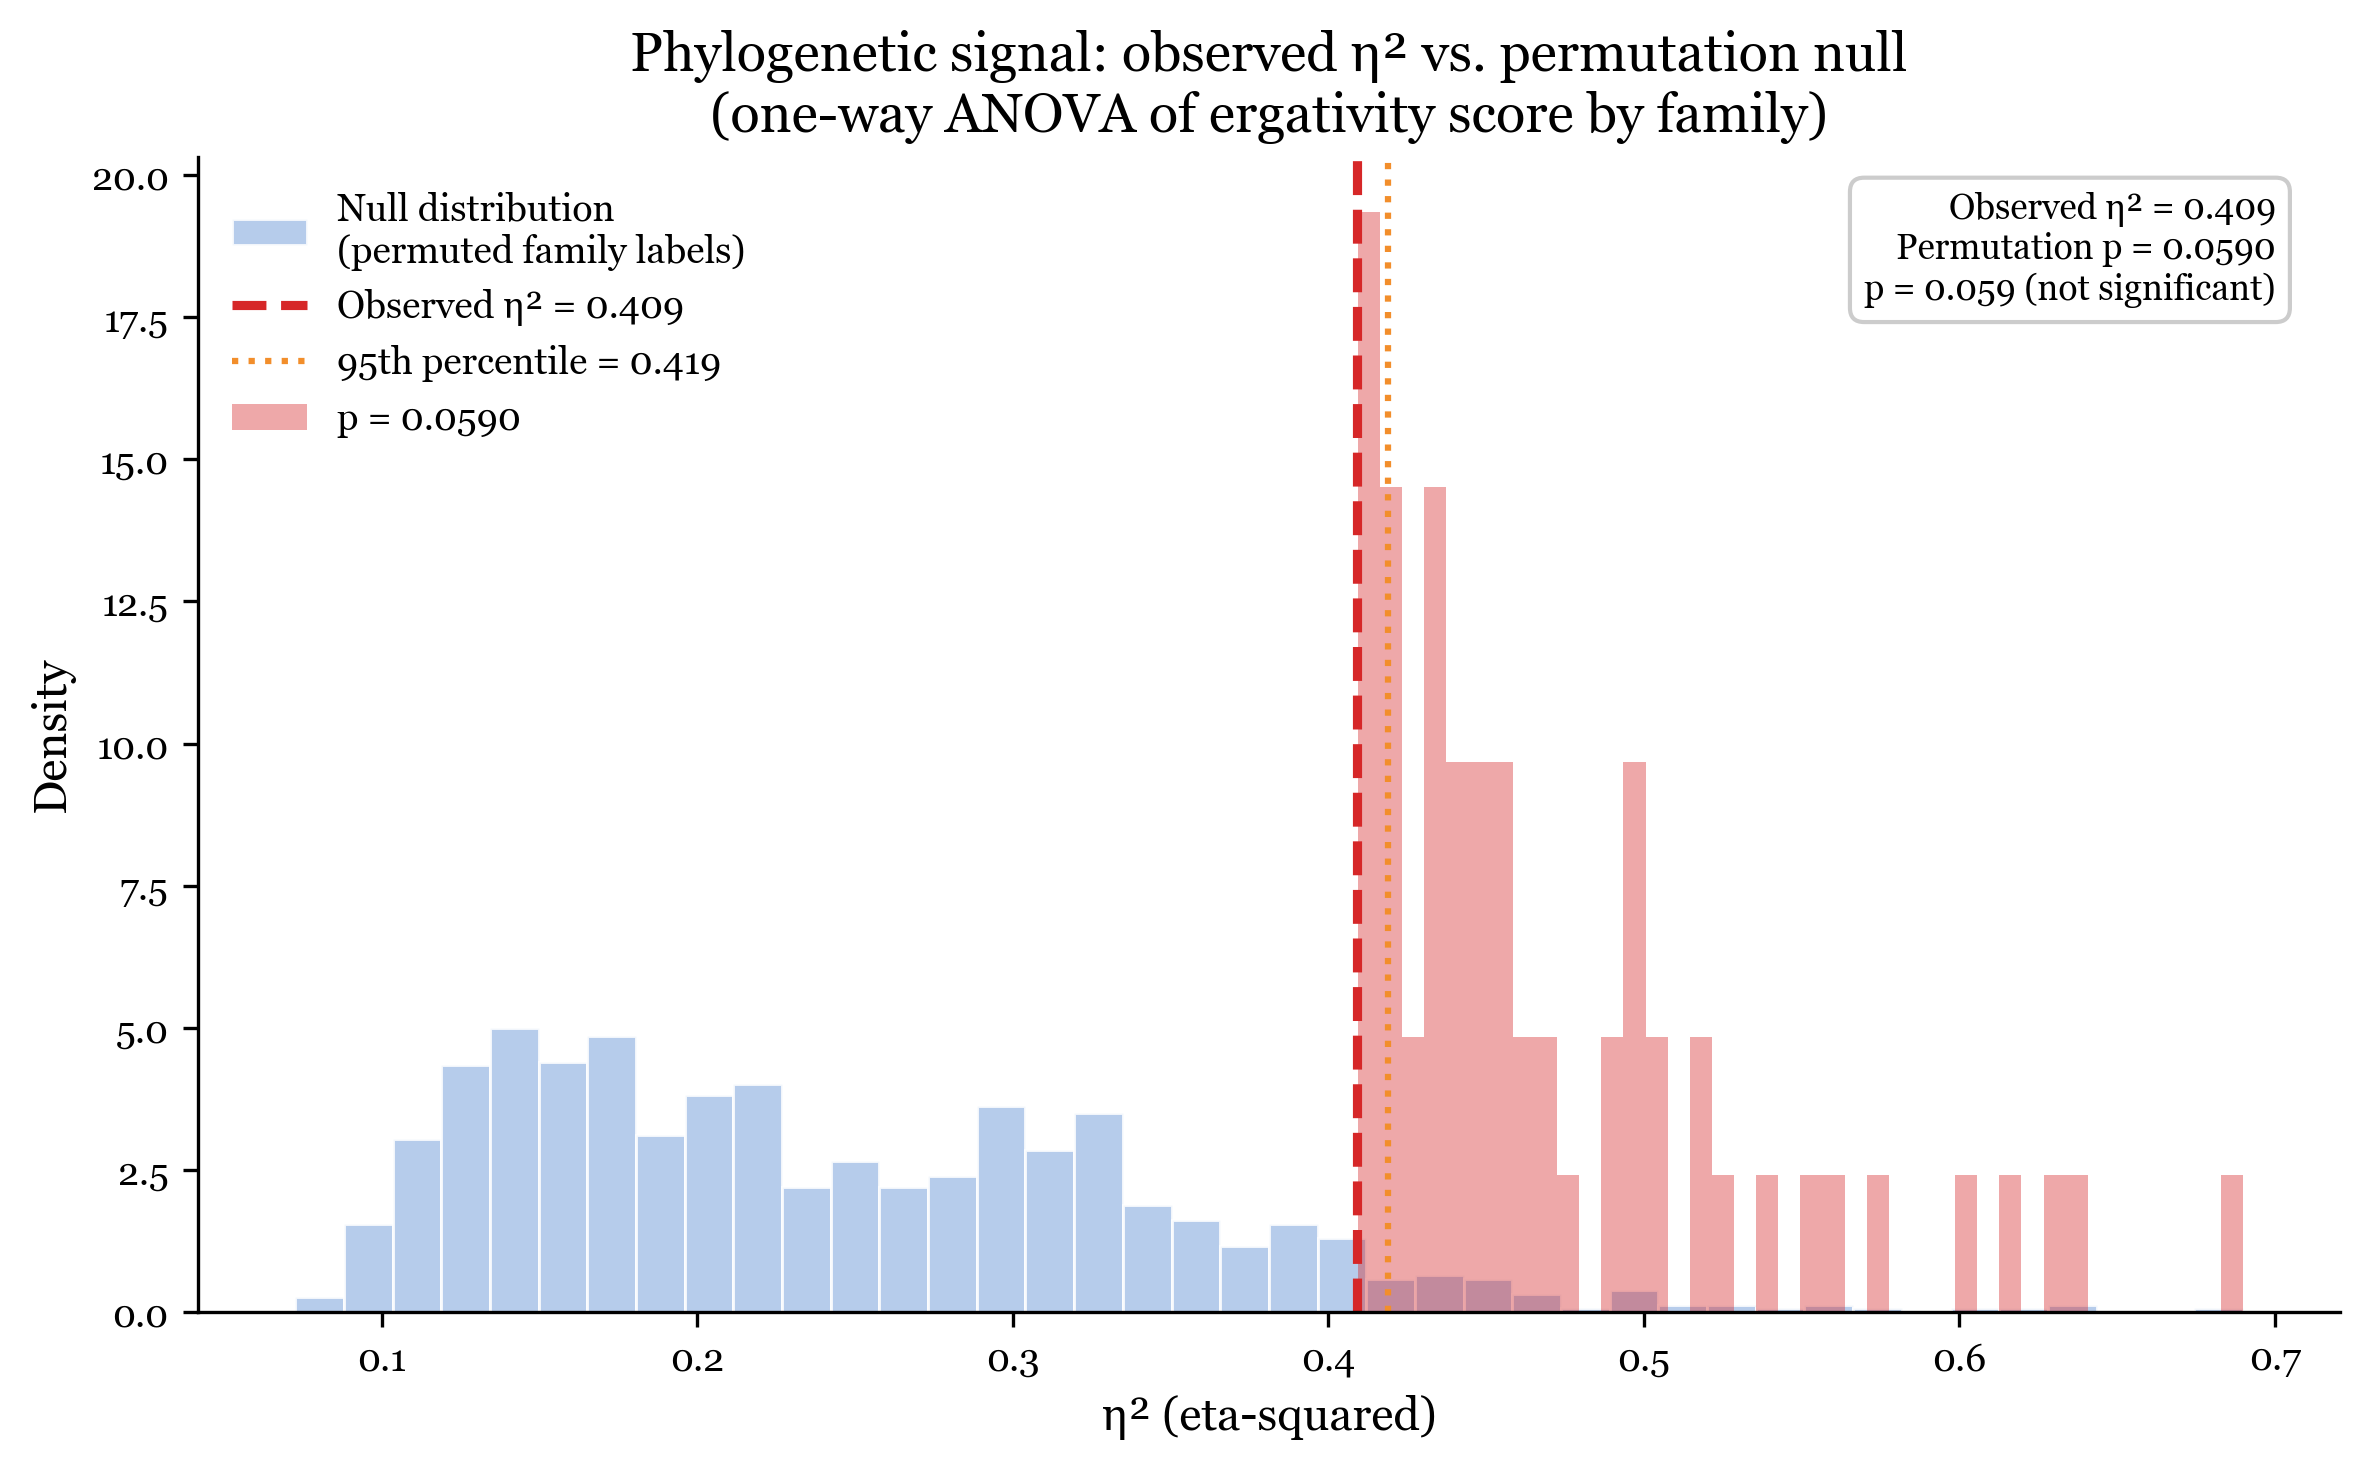
\includegraphics[width=0.82\textwidth]{figures/figA_phylogenetic_eta2.png}
  \caption{Permutation distribution of $F$-statistics (grey); observed $F$ in
    red.}
  \label{fig:eta2}
\end{figure}

\begin{figure}[H]
  \centering
  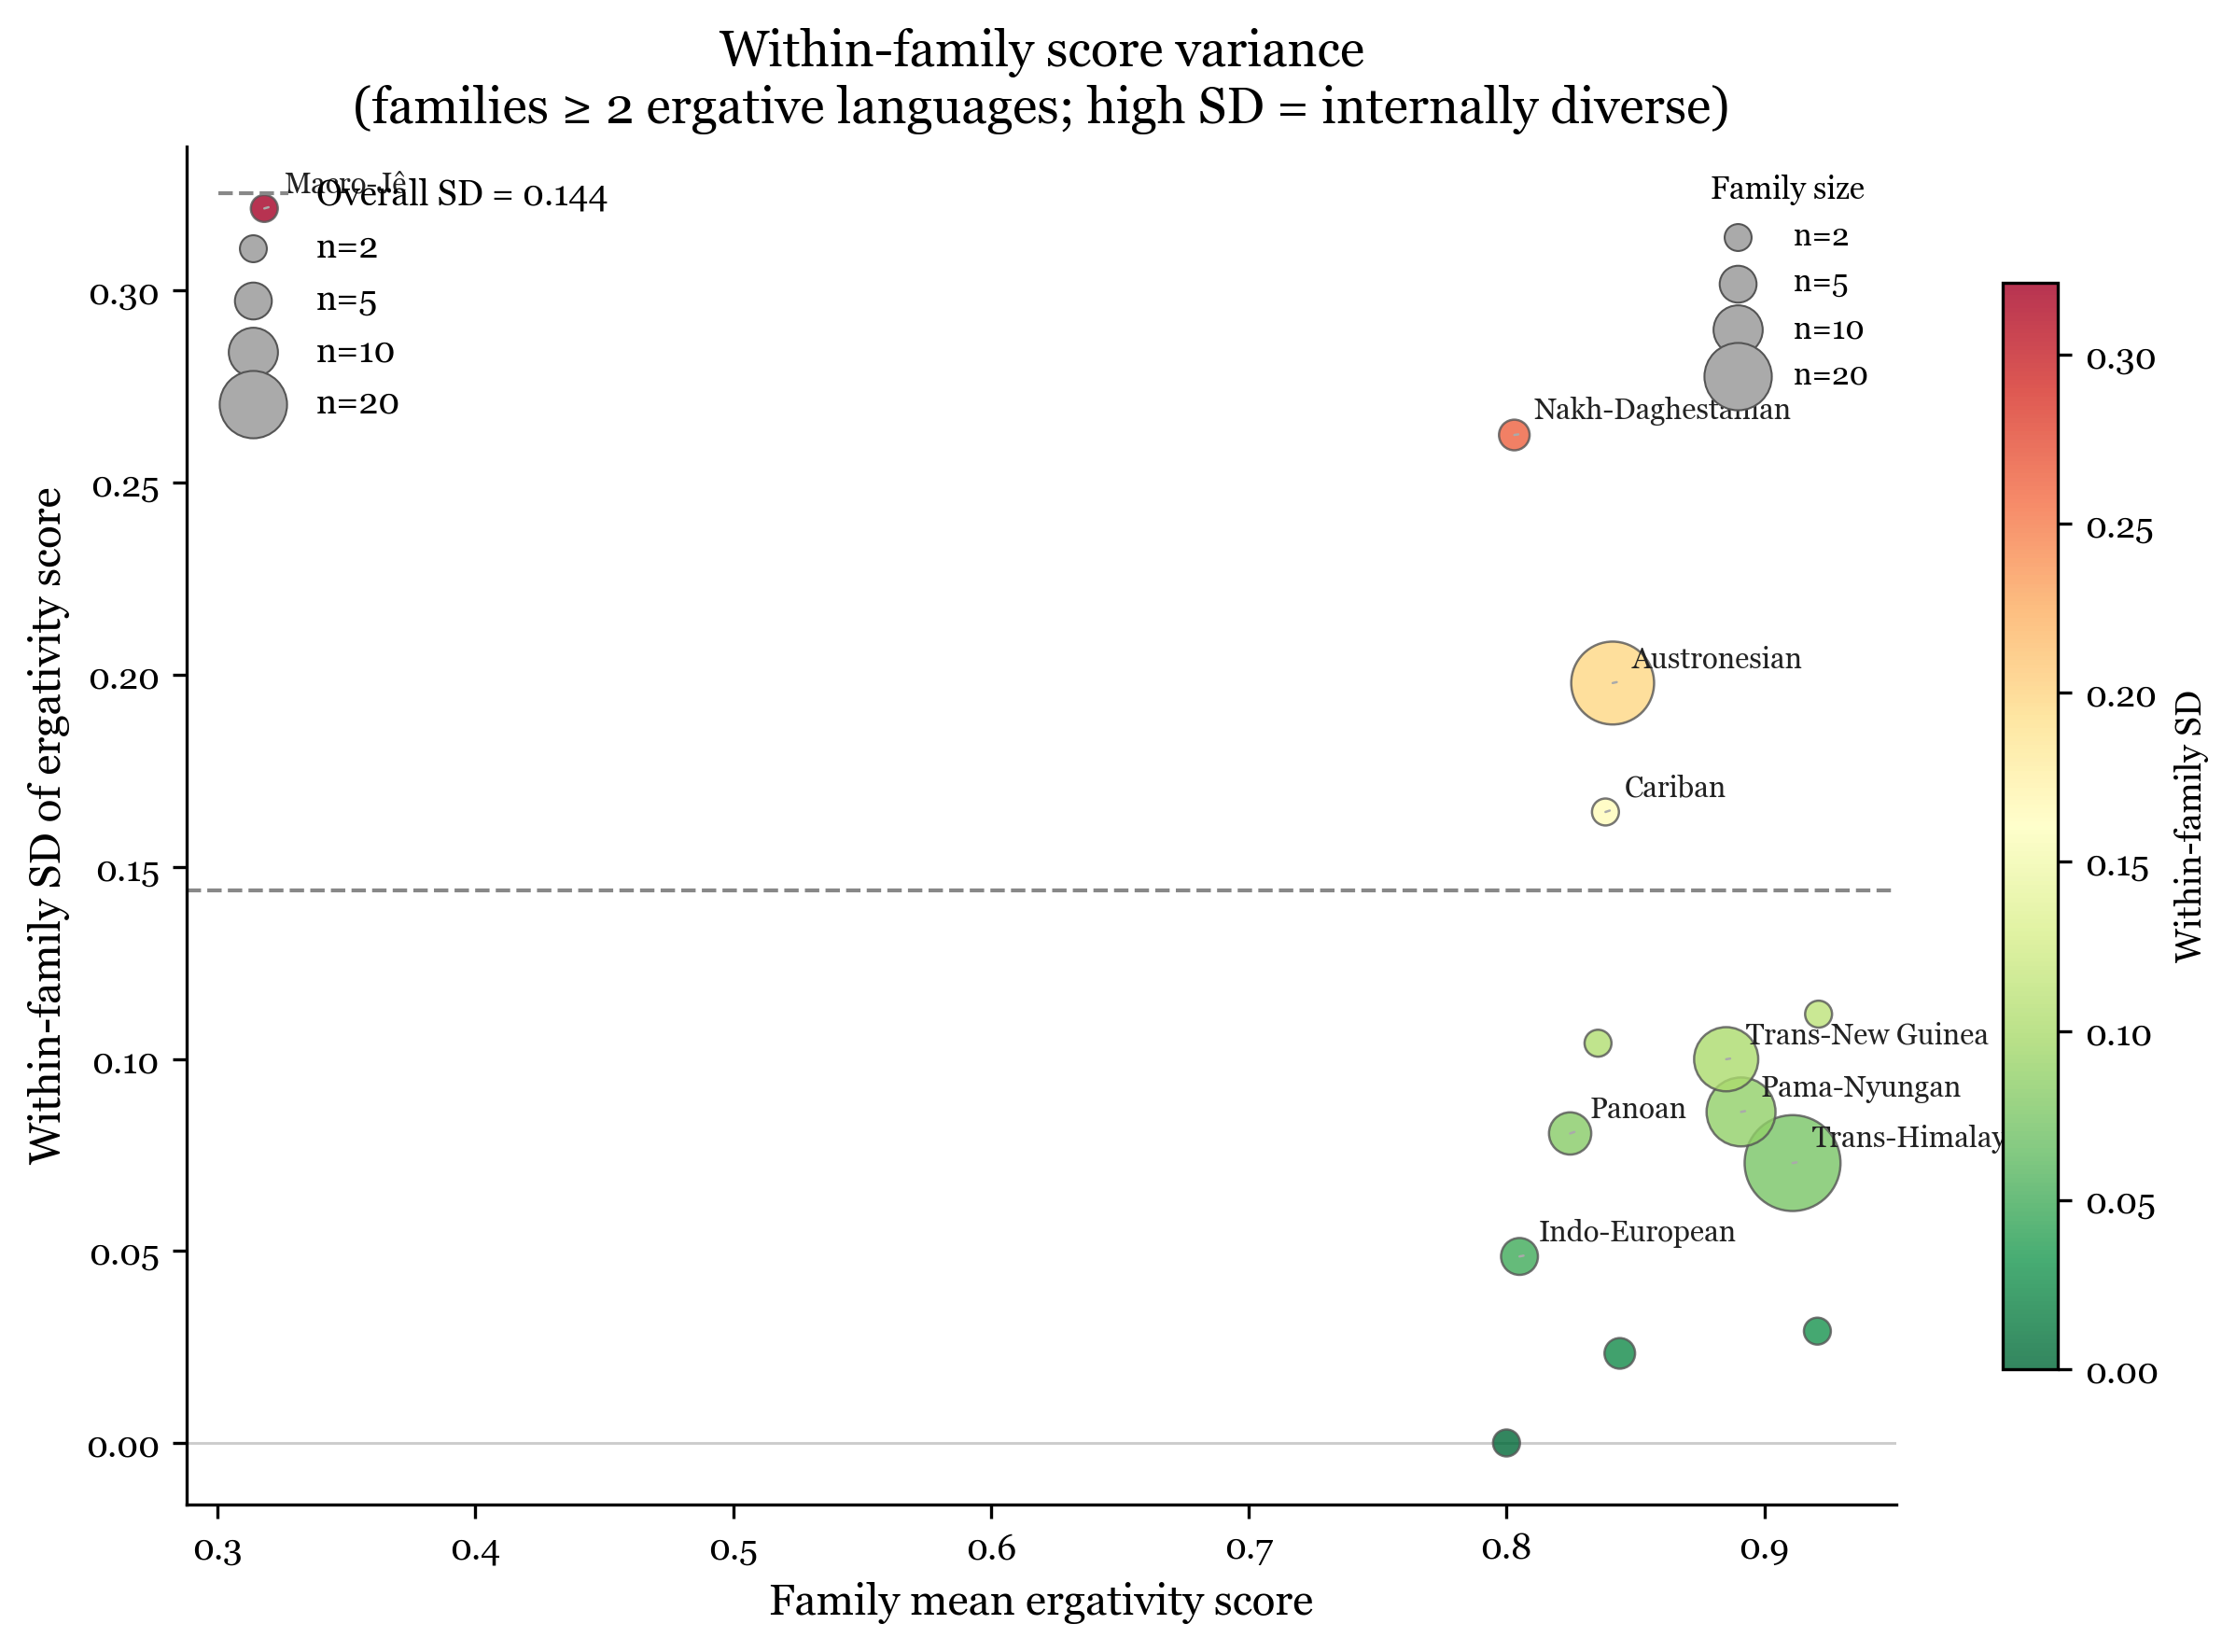
\includegraphics[width=0.82\textwidth]{figures/figB_within_family_variance.png}
  \caption{Within-family variance in ergativity scores. Each point is one family.}
  \label{fig:within_family}
\end{figure}

\begin{figure}[H]
  \centering
  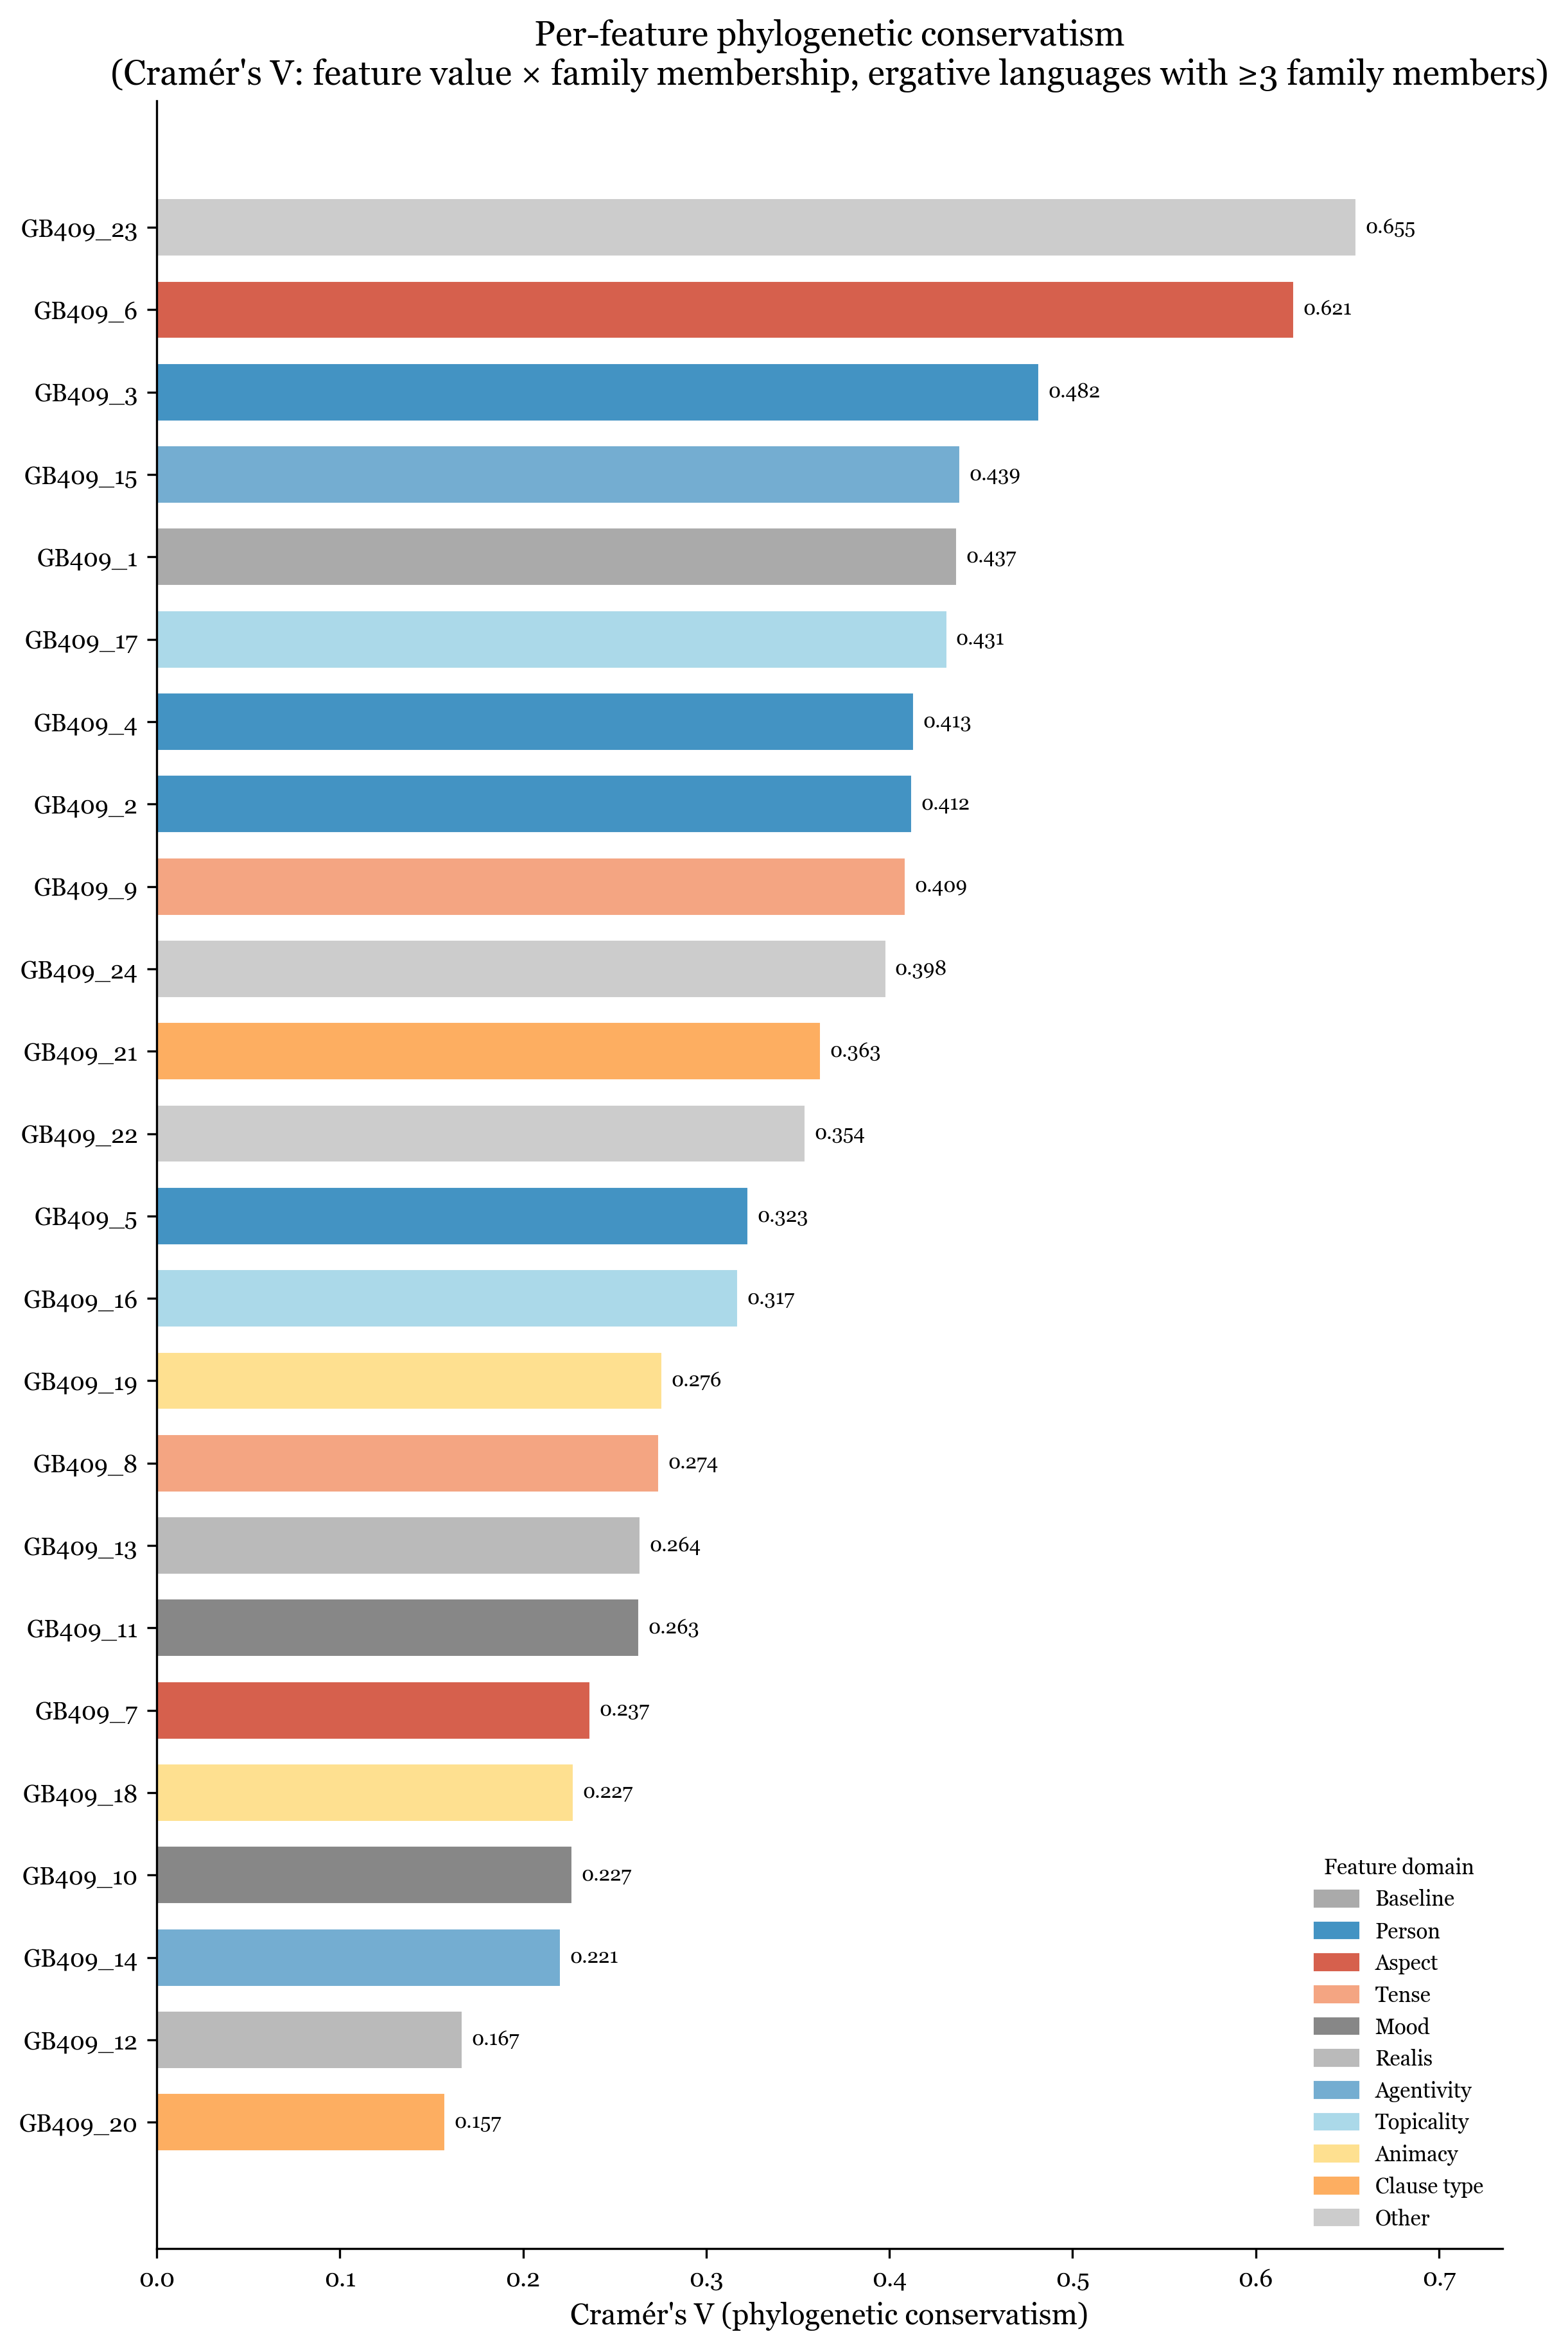
\includegraphics[width=0.82\textwidth]{figures/figC_feature_conservatism.png}
  \caption{Phylogenetic conservatism (Cram\'er's $V$) per feature, coloured by
    domain. Higher $V$ = more family-specific.}
  \label{fig:conservatism}
\end{figure}

% ══════════════════════════════════════════════════════════════════════════════
\section{Discussion}

Taken together, these seven analyses paint a coherent picture of ergativity as a
robust, pervasive, and partially genealogically constrained grammatical property.
Several findings stand out.

The distribution of ergativity scores ($M = 0.855$, $\mathrm{Mdn} = 0.900$) shows
that ERGON languages are overwhelmingly high-ergativity systems. The 16 languages
with perfect scores --- spanning Trans-Himalayan, Pama-Nyungan,
Chukotko-Kamchatkan, Salishan, and Trans-New Guinea --- represent the typological
prototype of ergativity. At the same time, the full range from 0.045 to 1.0
confirms that ergativity is a gradient property even among languages classified
as ergative.

The Silverstein hierarchy is remarkably well-respected (92.5\% conformance). The
12 violations are partly genealogically coherent: three of the four $[1,1,1,0]$
violators are Austronesian, suggesting that hierarchy violations, when they occur,
tend to be inherited rather than independently evolved.

The near-absence of unexpected splits ($< 2\%$ per domain) is a strong result. It
implies that in ERGON, ergativity is overwhelmingly a language-wide property. This
contrasts with a view of ergativity as primarily a split phenomenon driven by
aspect or tense --- a view that may be more applicable to different samples or to
morphosyntactic ergativity.

The extraordinary intercorrelation among tense, aspect, mood, and realis features
($\varphi > 0.97$) reveals that these conditioning environments are not
independent in the ERGON languages. A language that marks the ergative in the
perfective will, with near certainty, also mark it in the past, the indicative,
and the realis. This aligns with \citeauthor{bybee1994}'s
(\citeyear{bybee1994}) observation that these categories form a grammatical
coherence cluster.

The phylogenetic signal analysis ($\eta^2 \approx 0.41$) reveals that family
membership explains roughly 40\% of variance in ergativity patterns --- substantial,
but leaving 60\% to be explained by contact, drift, or functional pressures. The
differential conservatism of individual features invites further investigation into
diachronic pathways of ergativity change.

% ══════════════════════════════════════════════════════════════════════════════
\section{Conclusion}

This report has presented the first systematic quantitative analysis of the ERGON
database across 180 ergative languages. The results establish several robust
typological generalisations: ergativity is broadly deployed across conditioning
domains (mean 7.3/9 domains active); the Silverstein hierarchy is overwhelmingly
respected (92.5\%); split ergativity in unexpected directions is nearly absent;
tense, aspect, mood, and realis features form a tightly intercorrelated cluster
($\varphi > 0.97$) and are the strongest predictors of total ergativity score; and
roughly 40\% of cross-linguistic variation is genealogically determined.

Future work should expand the database to include the remaining Panoan and Takanan
languages currently missing from ERGON, and should explore syntactic ergativity as
a separate dimension. A geographic analysis examining whether ergativity clusters in
specific macro-areas beyond genealogical prediction would complement the
phylogenetic results reported here. Finally, the tight feature correlations within
the tense/aspect/mood/realis cluster raise the question of whether these should be
treated as a single latent variable in future statistical modelling.

% ══════════════════════════════════════════════════════════════════════════════
\bibliographystyle{apalike}
\bibliography{references}

\end{document}
